\documentclass{ieeeojies}
\usepackage{cite}
\usepackage{amsmath,amssymb,amsfonts}
\usepackage{algorithmic}
\usepackage{graphicx}
\usepackage{textcomp}
\usepackage{array}
\usepackage[table]{xcolor}
\usepackage{multirow}
\usepackage{multicol}
\usepackage{float}
\usepackage{ragged2e}
\usepackage[backend=bibtex,style=ieee]{biblatex} 
\addbibresource{Report.bib}

\def\BibTeX{{\rm B\kern-.05em{\sc i\kern-.025em b}\kern-.08em
    T\kern-.1667em\lower.7ex\hbox{E}\kern-.125emX}}

\begin{document}
\title{FORECASTING THE CURRENCY PRICE}

\author{\uppercase{Trinh Thi My Chung}\authorrefmark{1},
\uppercase{Tran Phuong Anh\authorrefmark{2}, and Che Duy Khang 3}\authorrefmark{3}}

\address[1]{Faculty of Information Systems, University of Information Technology, (e-mail: 21520653@gm.uit.edu.vn)}
\address[2]{Faculty of Information Systems, University of Information Technology, (e-mail: 21520595@gm.uit.edu.vn)}
\address[3]{Faculty of Information Systems, University of Information Technology, (e-mail: 21522187@gm.uit.edu.vn)}

\markboth
{Team 4 \headeretal: Trinh Thi My Chung, Tran Phuong Anh, Che Duy Khang}
{Team 4 \headeretal: Trinh Thi My Chung, Tran Phuong Anh, Che Duy Khang}

\begin{abstract}

The rapid fluctuations in currency exchange rates pose significant challenges for investors and policymakers. This study aims to forecast currency prices using a range of statistical, machine learning, and deep learning algorithms. The models employed in this research include Linear Regression, Autoregressive Integrated Moving Average (ARIMA), Exponential Smoothing State Space Model (ETS), Stacking model, Multilayer Perceptron (MLP), Recurrent Neural Networks (RNN), Gated Recurrent Units (GRU), and Long Short-Term Memory (LSTM). Evaluation metrics such as Mean Absolute Percentage Error (MAPE), Root Mean Squared Error (RMSE), and Mean Absolute Error (MAE) are utilized to assess the performance of each forecasting model on various currency datasets. The findings indicate that deep learning models, particularly GRU and LSTM, outperform other methods in predicting currency prices.
\end{abstract}

\begin{keywords}

\textit{\textbf{Key words:}} Forecasting the currency price, Linear Regression, Autoregressive Integrated Moving Average (ARIMA), Exponential Smoothing (ETS), Stacking model, Multilayer Perceptron (MLP), Recurrent Neural Networks (RNN), Gated Recurrent Units (GRU), Long Short-Term Memory (LSTM)
\end{keywords}

\titlepgskip=-15pt

\maketitle

\section{Introduction}
\label{sec:introduction}
\justify
Currency prices represent exchange rates between different currencies from different countries. Their fluctuations significantly impact various aspects of the global economy, including trade, investment and banking. This report focuses on time-series exchange rate forecasts between the Vietnamese Dong (VND) and Euro (EUR), British Pound (GBP) and Japanese Yen (JPY). Helps businesses manage risks and optimize profits, providing opportunities to improve forecasting capabilities, create competitive advantages and promote strategic development in the global business environment.

To analyze and forecast exchange rates between Vietnam and other countries, we use Linear Regression, ARIMA, Exponential Smoothing State Space Model (ETS), Stacking Model (XGBoost and Linear Regression), RNN, LSTM, GRU, MLP. Each model brings distinct strengths to the analysis, facilitating a thorough examination of the intricate dynamics shaping currency movements.

\section{Related Works}
\justify
Pengfei Liu et al. \cite{rw1} studied currency price prediction by implementing multiple forecasting models to forecast and analyze the daily currency price of USD/RMB. The research uses CNN, STLSTM, and AM model to estimate the model accuracy. Experiments show that all three models above have higher forecasting accuracy and coverage than other models and they are suitable for forecasting the closing price of the USD/RMB currency price.

Asadullah et al. \cite{rw2} forecast the future exchange rate values of the US Dollar (USD) against the Pakistani Rupee (PKR). The authors used the ARIMA model, and the time series data was stationary at first difference. After conducting the analysis, the difference between predicted and actual values is less than 0.01, which can be concluded that the ARIMA model is robust and can be a useful model in forecasting currency prices.

M.S. Islam and E.Hossain \cite{rw3} introduce a new model combining two advanced neural networks, Gate Recurrent Unit (GRU) and Long short-term memory in order to forecast future closing prices of foreign exchange currency, which are EUR/USD, GBP/USD, USD/CAD and USD/CHF. The model is built including a GRU layer with 20 hidden neurons as the first layer while an LSTM layer with 256 hidden neurons as the second layer

Qimian Zhu \cite{rw4} has an article forecasting the change in USD/EUR currency prices in 2022 using ARIMA model. Researchers discussed the performance of the univariate ARIMA model and the multivariate regression model with ARIMA errors, i.e. four macroeconomic variables, affecting the currency price incorporated in the AR part of the ARIMA model.

Escudero et al. \cite{rw5} studies on forecasting EUR/USD exchange rates, using three methods: ARIMA, Elman Neural Network (RNN) and LSTM. The dataset is divided into training and validation sets and after applying three models and calculating model accuracy, LSTM shows that it has the best performance in forecasting in the short term while Elman demonstrates the best predictions in the long term.

\section{Materials}
\subsection{Dataset}
\justify
This study will utilize historical exchange rate data of Euro (EUR) to Vietnamese Dong (VND), British Pound (GBP) to Vietnamese Dong (VND), and Japanese Yen (JPY) to Vietnamese Dong (VND) from March 1, 2019, to June 1, 2024. The dataset includes columns such as Date, Purchase Price, Sale Price, and Transfer Price. Since the objective is to forecast foreign currencies' sale prices, only data related to the Sale (VND) columns will be processed.

\subsection{Descriptive Statistics}
\begin{table}[H]
  \centering
  \caption{EUR-VND, GBP-VND, JPY-VND dataset’s Descriptive Statistics}
\begin{tabular}{|>{\columncolor{red!20}}c|c|c|c|}
    \hline
     \rowcolor{red!20} & EUR-VND & GBP-VND & JPY-VND \\ \hline
     Count & 1920 & 1920 & 1920 \\ \hline
     Mean & 26775.5 & 30508.5 & 199.3\\ \hline
     Std & 1072.64 & 1315.09 & 20.92\\ \hline
     Min & 23533 & 25979 & 166.16\\ \hline
     25\% & 26176 & 29590 & 176.83\\ \hline
     50\% & 26681 & 30501 & 207.67\\ \hline
     75\% & 27607.5 & 31521 & 217.58\\ \hline
     Max & 29180 & 33305 & 228.6\\ \hline
\end{tabular}
\end{table}

\begin{figure}[H]
    \centering
    \begin{minipage}{0.23\textwidth}
    \centering
    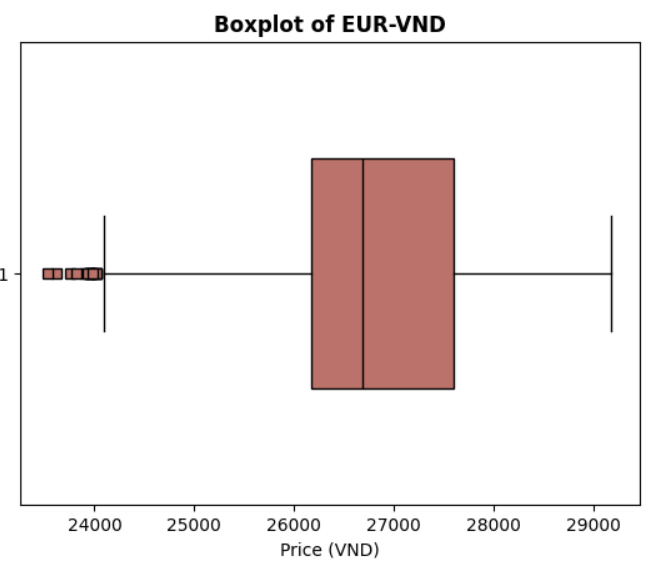
\includegraphics[width=1\textwidth]{Descriptive_statistic/eur_boxplot.png}
    \caption{EUR-VND price's boxplot}
    \label{fig:1}
    \end{minipage}
    \hfill
    \begin{minipage}{0.23\textwidth}
    \centering
    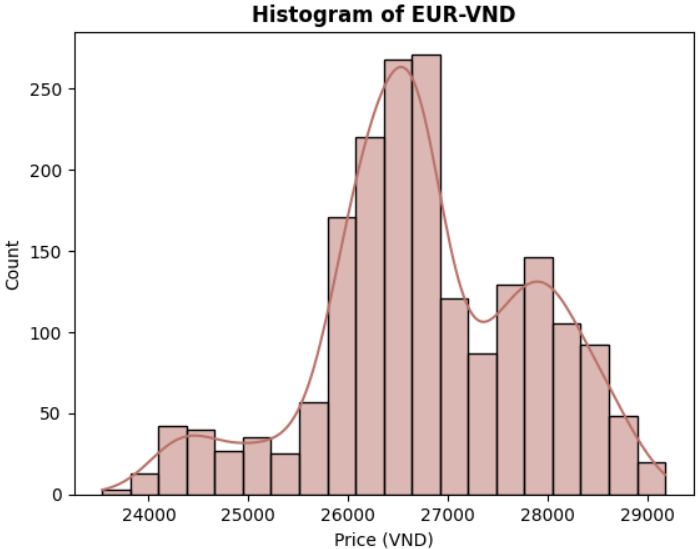
\includegraphics[width=1\textwidth]{Descriptive_statistic/eur_histogram.png}
    \caption{EUR-VND price's histogram}
    \label{fig:2}
    \end{minipage}
\end{figure}
\justify
From the descriptive statistics of the EUR-VND dataset, we can observe that the selling price of the Euro (EUR) to Vietnamese Dong (VND) currency pair from March 1, 2019, to June 1, 2024, exhibits a skewed distribution with the primary concentration around the mean and median values, but with uneven fluctuations.
\begin{figure}[H]
    \centering
    \begin{minipage}{0.23\textwidth}
    \centering
    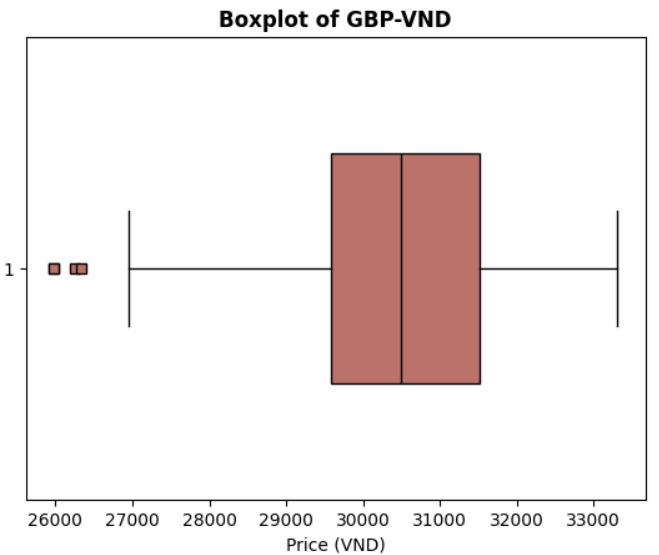
\includegraphics[width=1\textwidth]{Descriptive_statistic/gbp_boxplot.png}
    \caption{GBP-VND price's boxplot}
    \label{fig:1}
    \end{minipage}
    \hfill
    \begin{minipage}{0.23\textwidth}
    \centering
    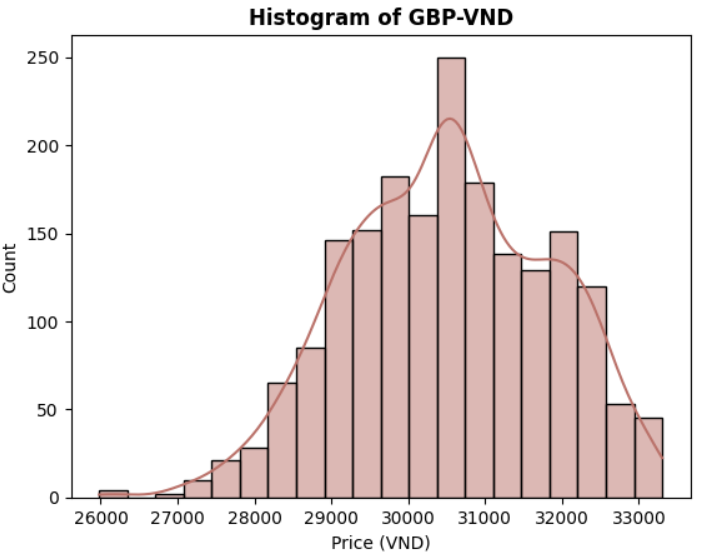
\includegraphics[width=1\textwidth]{Descriptive_statistic/gbp_histogram.png}
    \caption{GBP-VND price's histogram}
    \label{fig:2}
    \end{minipage}
\end{figure}
\justify
From the descriptive statistics of the GBP-VND dataset, we can observe a certain level of volatility in the selling prices of the British Pound (GBP) to Vietnamese Dong (VND) currency pair from March 1, 2019, to June 1, 2024. Most selling prices are concentrated at lower levels, with some higher values contributing to an increase in standard deviation and causing a skewed right distribution on the histogram. 
\begin{figure}[H]
    \centering
    \begin{minipage}{0.23\textwidth}
    \centering
    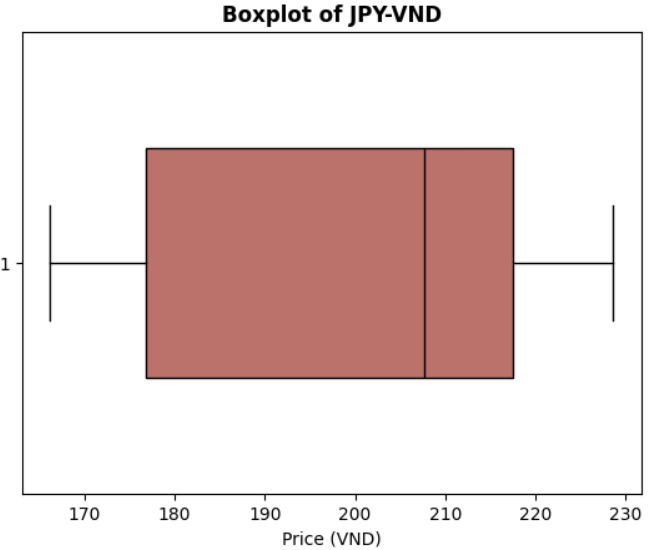
\includegraphics[width=1\textwidth]{Descriptive_statistic/jpy_boxplot.png}
    \caption{JPY-VND price's boxplot}
    \label{fig:1}
    \end{minipage}
    \hfill
    \begin{minipage}{0.23\textwidth}
    \centering
    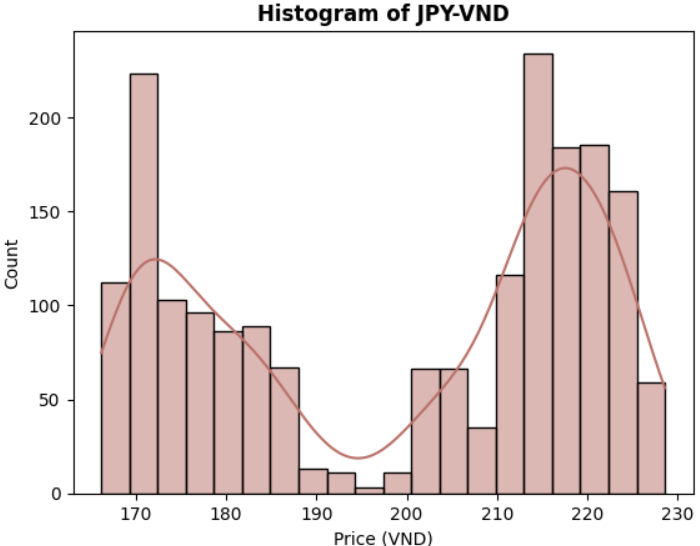
\includegraphics[width=1\textwidth]{Descriptive_statistic/jpy_histogram.png}
    \caption{JPY-VND price's histogram}
    \label{fig:2}
    \end{minipage}
\end{figure}
\justify
From the descriptive statistics of the JPY-VND dataset, we can observe that the market selling price of the Japanese Yen (JPY) to Vietnamese Dong (VND) from March 1, 2019, to June 1, 2024, exhibits variability and fluctuations. The histogram of the data indicates instability and variability in the values. The boxplot of the dataset reveals that the majority of values concentrate at higher price levels.

\section{Methodology}
\subsection{Linear Regression}
Regression analysis is a tool for building mathematical and statistical models that characterize relationships between a dependent variable and one or more independent, or explanatory, variables, all of which are numerical. This statistical technique is used to find an equation that best predicts the y variable as a linear function of the x variables.
A multiple linear regression model has the form: 
\[Y=\beta_0+\beta_1X_1+\beta_2X_2+\cdots+\beta_kX_k+\varepsilon\]
Where:
\begin{itemize}
	\item $Y$ is the dependent variable (Target Variable).
	\item $X_1, X_2, \ldots, X_k$ are the independent (explanatory) variables.
	\item $\beta_0$ is the intercept term.
	\item $\beta_1,..., \beta_k$ are the regression coefficients for the independent variables.
	\item $\varepsilon$ is the error term. \cite{linear}
 \end{itemize}

 \subsection{AutoRegressive Integrated Moving Average (ARIMA)}
 ARIMA model is a form of regression analysis that gauges the strength of one dependent variable relative to other changing variables. The ARIMA model is used to make predictions about future values of the time series based on its past values. The ARIMA model consists of three parts including Autoregressive (AR), Integrated (I), and Moving Average (MA). \cite{investopedia_arima} \par
\noindent
 The AR component with order p utilizes the preceding p values of the time series for current value prediction. The AR(p) model has the form:
 \[Y_t=\alpha_0+\alpha_1Y_{t-1}+\cdots+\alpha_pY_{t-p}+\epsilon_t\]
Where:
    \begin{itemize}
	\item $Y_t$ is the current observed value.
        \item $Y_{t-1}, \ldots, Y_{t-p}$ are past observed values.
        \item $\alpha_0, \alpha_1, \ldots, \alpha_p$ are regression analysis parameters.
        \item $\epsilon_t$ is the random forecasting error of the current period. The expected mean value is 0.
    \end{itemize}
 Integrated (I) represents the differencing of raw observations, allowing the time series to become stationary.
 \begin{itemize}
    \item First Difference I(1): $dY_t = Y_t - Y_{t-1}$
    \item Second Difference I(2): $dY_t = Y_t - 2Y_{t-2} + Y_{t-3}$
 \end{itemize}
The MA model with order q analyzes the past q forecast errors to anticipate the current value. The MA(q) model has the form:
  \[Y_t=\beta_0+\epsilon_t+\beta_1\epsilon_{t-1}+\cdots+\beta_q\epsilon_{t-q}\]
        Where:
        \begin{itemize}
	    \item $Y_t$ is the current observed value.
            \item $\epsilon_t$ is a random forecasting error of the current period. The expected mean value is 0.
            \item \(\epsilon_{t-1}, \ldots, \epsilon_{t-q}\) are forecast errors.
            \item \(\beta_0, \beta_1, \ldots, \beta_q\) mean values of Y(t) and moving average coefficients.
            \cite{arima_forecasting}
        \end{itemize}
            
\subsection{Exponential Smoothing (ETS)}
Exponential smoothing is one of the most popular models used for demand forecasting in practice. It includes Error, Trend, and Seasonal components, thus being called ‘ETS’.
The trend component (T) represents the tendency to increase or decrease data over time. The seasonal (S) shows the periodic fluctuations at fixed intervals within the data. The fluctuations are affected by specific times of the year like holidays, seasonal changes, or events. The error (E) is also known as residual. It represents the unpredictable or fluctuations in the data that cannot be explained by the trend or seasonal components.
There are three main methods to estimate exponential smoothing, which are: \\
    \indent\textbullet\ Simple exponential smoothing: used when the data has no trend and no seasonal pattern. \\
    \indent\textbullet\ Double exponential smoothing: used for forecasting the time series when the data has a linear trend and no seasonal pattern. \\
    \indent\textbullet\ Triple exponential smoothing: used for forecasting the time series when the data has both linear trend and seasonal pattern. This method is also called Holt-Winters exponential smoothing \cite{ets_triple}
    \begin{align*}
        L_t &= \alpha(Y_t - S_{t-p}) + (1 - \alpha)(L_{t-1} + T_{t-1}) \\
        T_t &= \beta(L_t - L_{t-1}) + (1 - \beta)T_{t-1} \\
        S_t &= \delta(Y_t - L_t) + (1 - \delta)S_{t-p} \\
        \hat{Y}_t &= L_{t-1} + T_{t-1} + S_{t-p}
    \end{align*} 
    \begin{itemize}
      \item $\alpha$, $\beta$, $\gamma$ : smoothing parameters
      \item $Y_t$ : actual data point at time $t$
      \item $S_{t-p}$ : seasonal index at time $t-p$
      \item $T_{t-1}$ : trend at time $t-1$
      \item $L_{t-1}$: the level at time $t-1$
      \item $L$: the level at time $t$
      \item $\hat{Y}_t$: the forecast value at time $t$ \cite{ets_triple_formula}
    \end{itemize}

\subsection{Stacking model} 
The Stacking Model, also known as Ensemble Learning, is a machine learning technique that combines multiple machine learning models to create a more accurate predictive model, flexible and effective approach to solving complex prediction tasks. In general, stacking ensemble learning consists of two phases: base models training phase and meta model training phase:\

In the initial phase, the original data is first split into a training set and a testing set. The training set undergoes training using k-fold cross-validation. This method involves partitioning the training set into k subsets, using k minus one subsets for training the model, and predicting outcomes for the remaining subset.

During the subsequent phase, predictions from the k-fold cross-validation of the base model are aggregated to reconstruct a new training dataset in the original order. The meta model's training set is formed by consolidating these reconstructed datasets from multiple base models. Similarly, predictions from the testing sets of the base models are combined to construct the testing set for the meta model. The meta model is then trained

\begin{figure}[H]
  \centering
  \begin{minipage}{1.0\linewidth}
    \centering
    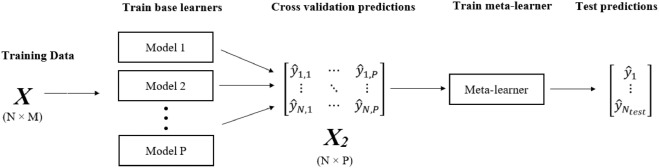
\includegraphics[width=\linewidth]{Figure_algorithm/stackingmodel.jpg}
    \caption{Structure of the Stacking Model \cite{stack_fig}}
  \end{minipage}
\end{figure}

In this report, two models XGBoost, Linear Regerssion  were selected as the base models. The meta-model was chosen as ordinary linear regression. Linear regression is a common choice in regression for the meta-learner

\subsection{XGBoost (For Stacking Model)}
Extreme Gradient Boosting (XGB) is an advanced supervised learning algorithm proposed by Chen and Guestrin. It is based on gradient-boosted decision trees and aims to create a strong learner by aggregating predictions from weak learners using additive training strategies. XGB builds upon gradient-boosted decision trees with a second-order Taylor expansion of the loss function and regularization to prevent overfitting and accelerate convergence. It continuously improves prediction accuracy by iteratively constructing new decision trees to fit residuals from previous predictions, minimizing the difference between predicted and actual values. Its speed advantage makes XGB a preferred choice as a base model for staking model in various studies.\cite{stacking}

\subsection{Recurrent Neural Network (RNN)}
RNN is a type of neural network model designed to handle sequential data. The distinctive feature of RNNs is their ability to maintain information across time steps, allowing them to utilize information from previous steps to influence the processing of the current step. This makes RNNs particularly useful in applications where the order of data is important, such as natural language processing (NLP), machine translation, and time series forecasting. \cite{zargar2021introduction}\\
RNNs operate by processing sequential data and maintaining a hidden state to capture information from previous time steps. The formula for updating the hidden state is:
\[ \alpha_t=\psi_0(W_\alpha_xx_t + W_\alpha_\alpha\alpha_t_-_1 + b_\alpha) \]

Where:\\
    \begin{itemize}
        \item $\alpha_t$ is a hidden layer state at each time step t
        \item $\psi_0$ is the activation function
        \item $W_\alpha_x$ and $W_\alpha_\alpha$ are weight matrices
        \item $x_t$ is an input data
        \item $b_\alpha$ is a bias vector
    \end{itemize}\\

The formula predicts the output at each time t:\\
\[ y_t = \Psi_1(W_y_\alpha\alpha_t + b_y) \]

Where:\\
    \begin{itemize}
        \item $y_t$ is an output data at each time t
        \item $\Psi_1$ is the activation function
        \item $W_y_\alpha$ is weight matrices
        \item $\alpha_t$ is a hidden layer state
        \item $b_y$ is a bias vector
        \cite{zargar2021introduction}
    \end{itemize}

\subsection{Gated Recurrent Unit (GRU)} 
Gated Recurrent Unit (GRU) is a special kind of RNN (Recurrent Neural Network). A GRU cell consists of two gates: the Update gate and the Reset gate. The Update gate operates similarly to the forget gate and input gate of LSTM. It determines how much of the past information to keep and how much new information from the current input to allow into cell state by controlling balance between the previous hidden state and the candidate hidden state \cite{gru_balance}. The Reset gate identifies and forgets unnecessary past information from the GRU network.

The equation of Update gate is as follows:
\begin{align*}
z_t &= \sigma\left( W^{(z)} x_t + U^{(z)} h_{t-1} \right)
\end{align*}

The equation of Reset gate is as follows:
\begin{align*}
r_t &= \sigma\left( W^{(r)} x_t + U^{(r)} h_{t-1} \right)
\end{align*}

Candidate hidden state is calculated from the reset gate and stores information from the past. Its equation is as follows:
\begin{align*}
h_t' &= \tanh(W \mathbf{x}_t + r_t \odot U \mathbf{h}_{t-1})
\end{align*}

The equation of Hidden state is as follows:
\begin{align*}
h_t &= z_t \odot h_{t-1} + (1 - z_t) \odot h_t'  
\end{align*}

Where:\\
    \begin{itemize}
        \item \(h_{t-1}\) represent the output of the previous states
        \item \(z_t\) is the update gate at time \(t\)
        \item \(r_t\) is the reset gate at time \(t\)
        \item \(W_z\), \(W_r\) is the weight matrix
        \item \(h_t\) is the hidden state at time \(t\)
        \item \(h_t'\) is the candidate hidden state at time \(t\)
        \item \(\sigma\) is the logistic sigmoid function \cite{gru_equation} \\
    \end{itemize}\\

\subsection{Long Short-Term Memory (LSTM)} 
The LSTM (Long Short-Term Memory) model, a specialized form of Recurrent Neural Network (RNN), was introduced by Hochreiter and Schmidhuber in 1997 to tackle the issue of long-term dependencies. It consists of a chain-like structure with up to four interacting layers. Each LSTM includes a cell state and three gates: forget, input, and output. These gates are controlled by sigmoid layers.\cite{zargar2021introduction}
\begin{figure}[H]
  \centering
  \begin{minipage}{0.8\linewidth}
    \centering
    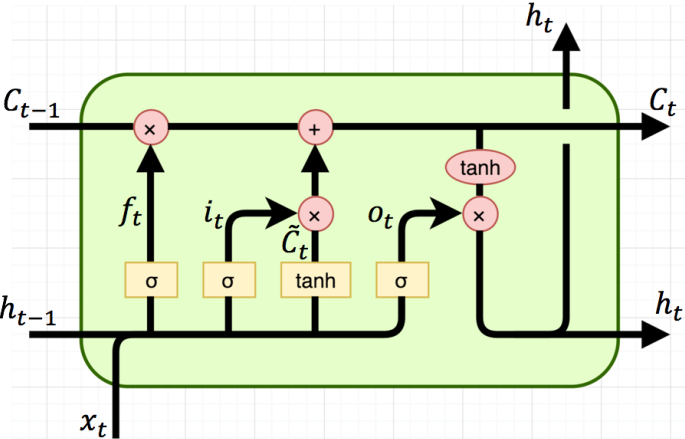
\includegraphics[width=\linewidth]{Figure_algorithm/lstm (1).png}
    \caption{Structure of the LSTM model \cite{lstm_fig}}
  \end{minipage}
\end{figure}
The initial step of the LSTM model involves the forget gate layer, which decides what information to discard from the cell state. The formula for the forget gate is:
\[ f_t = \sigma(W_f \cdot [h_{t-1}, x_t] + b_f) \]
Where:
\begin{itemize}
    \item \( \sigma \) is the sigmoid function.
    \item \( W_f \) and \( b_f \) are the weights and bias of the forget gate layer.
\end{itemize}

Subsequent steps determine which information is stored in and updates the cell state. This involves an input gate layer and a vector of values from the tanh layer. The formulas for the input gate and state update are:
\begin{align*}
    i_t & = \sigma(W_i \cdot [h_{t-1}, x_t] + b_i) \\
    \tilde{C}_t & = \tanh(W_C \cdot [h_{t-1}, x_t] + b_C) \\
    C_t & = f_t \cdot C_{t-1} + i_t \cdot \tilde{C}_t
\end{align*}
Where:
\begin{itemize}
    \item \( C_{t-1} \) and \( C_t \) are the cell states at time \( t-1 \) and \( t \)
    \item \( W_i, W_C \), and their respective variables are weights,
\end{itemize}

Finally, the output \( h_t \) is determined by the output gate and the cell state. The formula for the output gate is:
\begin{align*}
    o_t & = \sigma(W_o \cdot [h_{t-1}, x_t] + b_o) \\
    h_t & = o_t \cdot \tanh(C_t)
\end{align*}

\subsection{Multilayer Perceptron (MLP)}
MLP is a type of artificial neural network that belongs to the feed-forward neural network group. It consists of multiple layers: an input layer, one or more hidden layers, and an output layer. Each neuron in an MLP uses a nonlinear activation function, such as the sigmoid, ReLU, or tanh function. These neurons are fully connected, meaning each neuron in one layer is connected to every neuron in the adjacent layer. MLP can learn and model nonlinear relationships between inputs and outputs, making it effective for many complex problems. \cite{mlp}

\begin{figure}[H]
  \centering
  \begin{minipage}{0.8\linewidth}
    \centering
    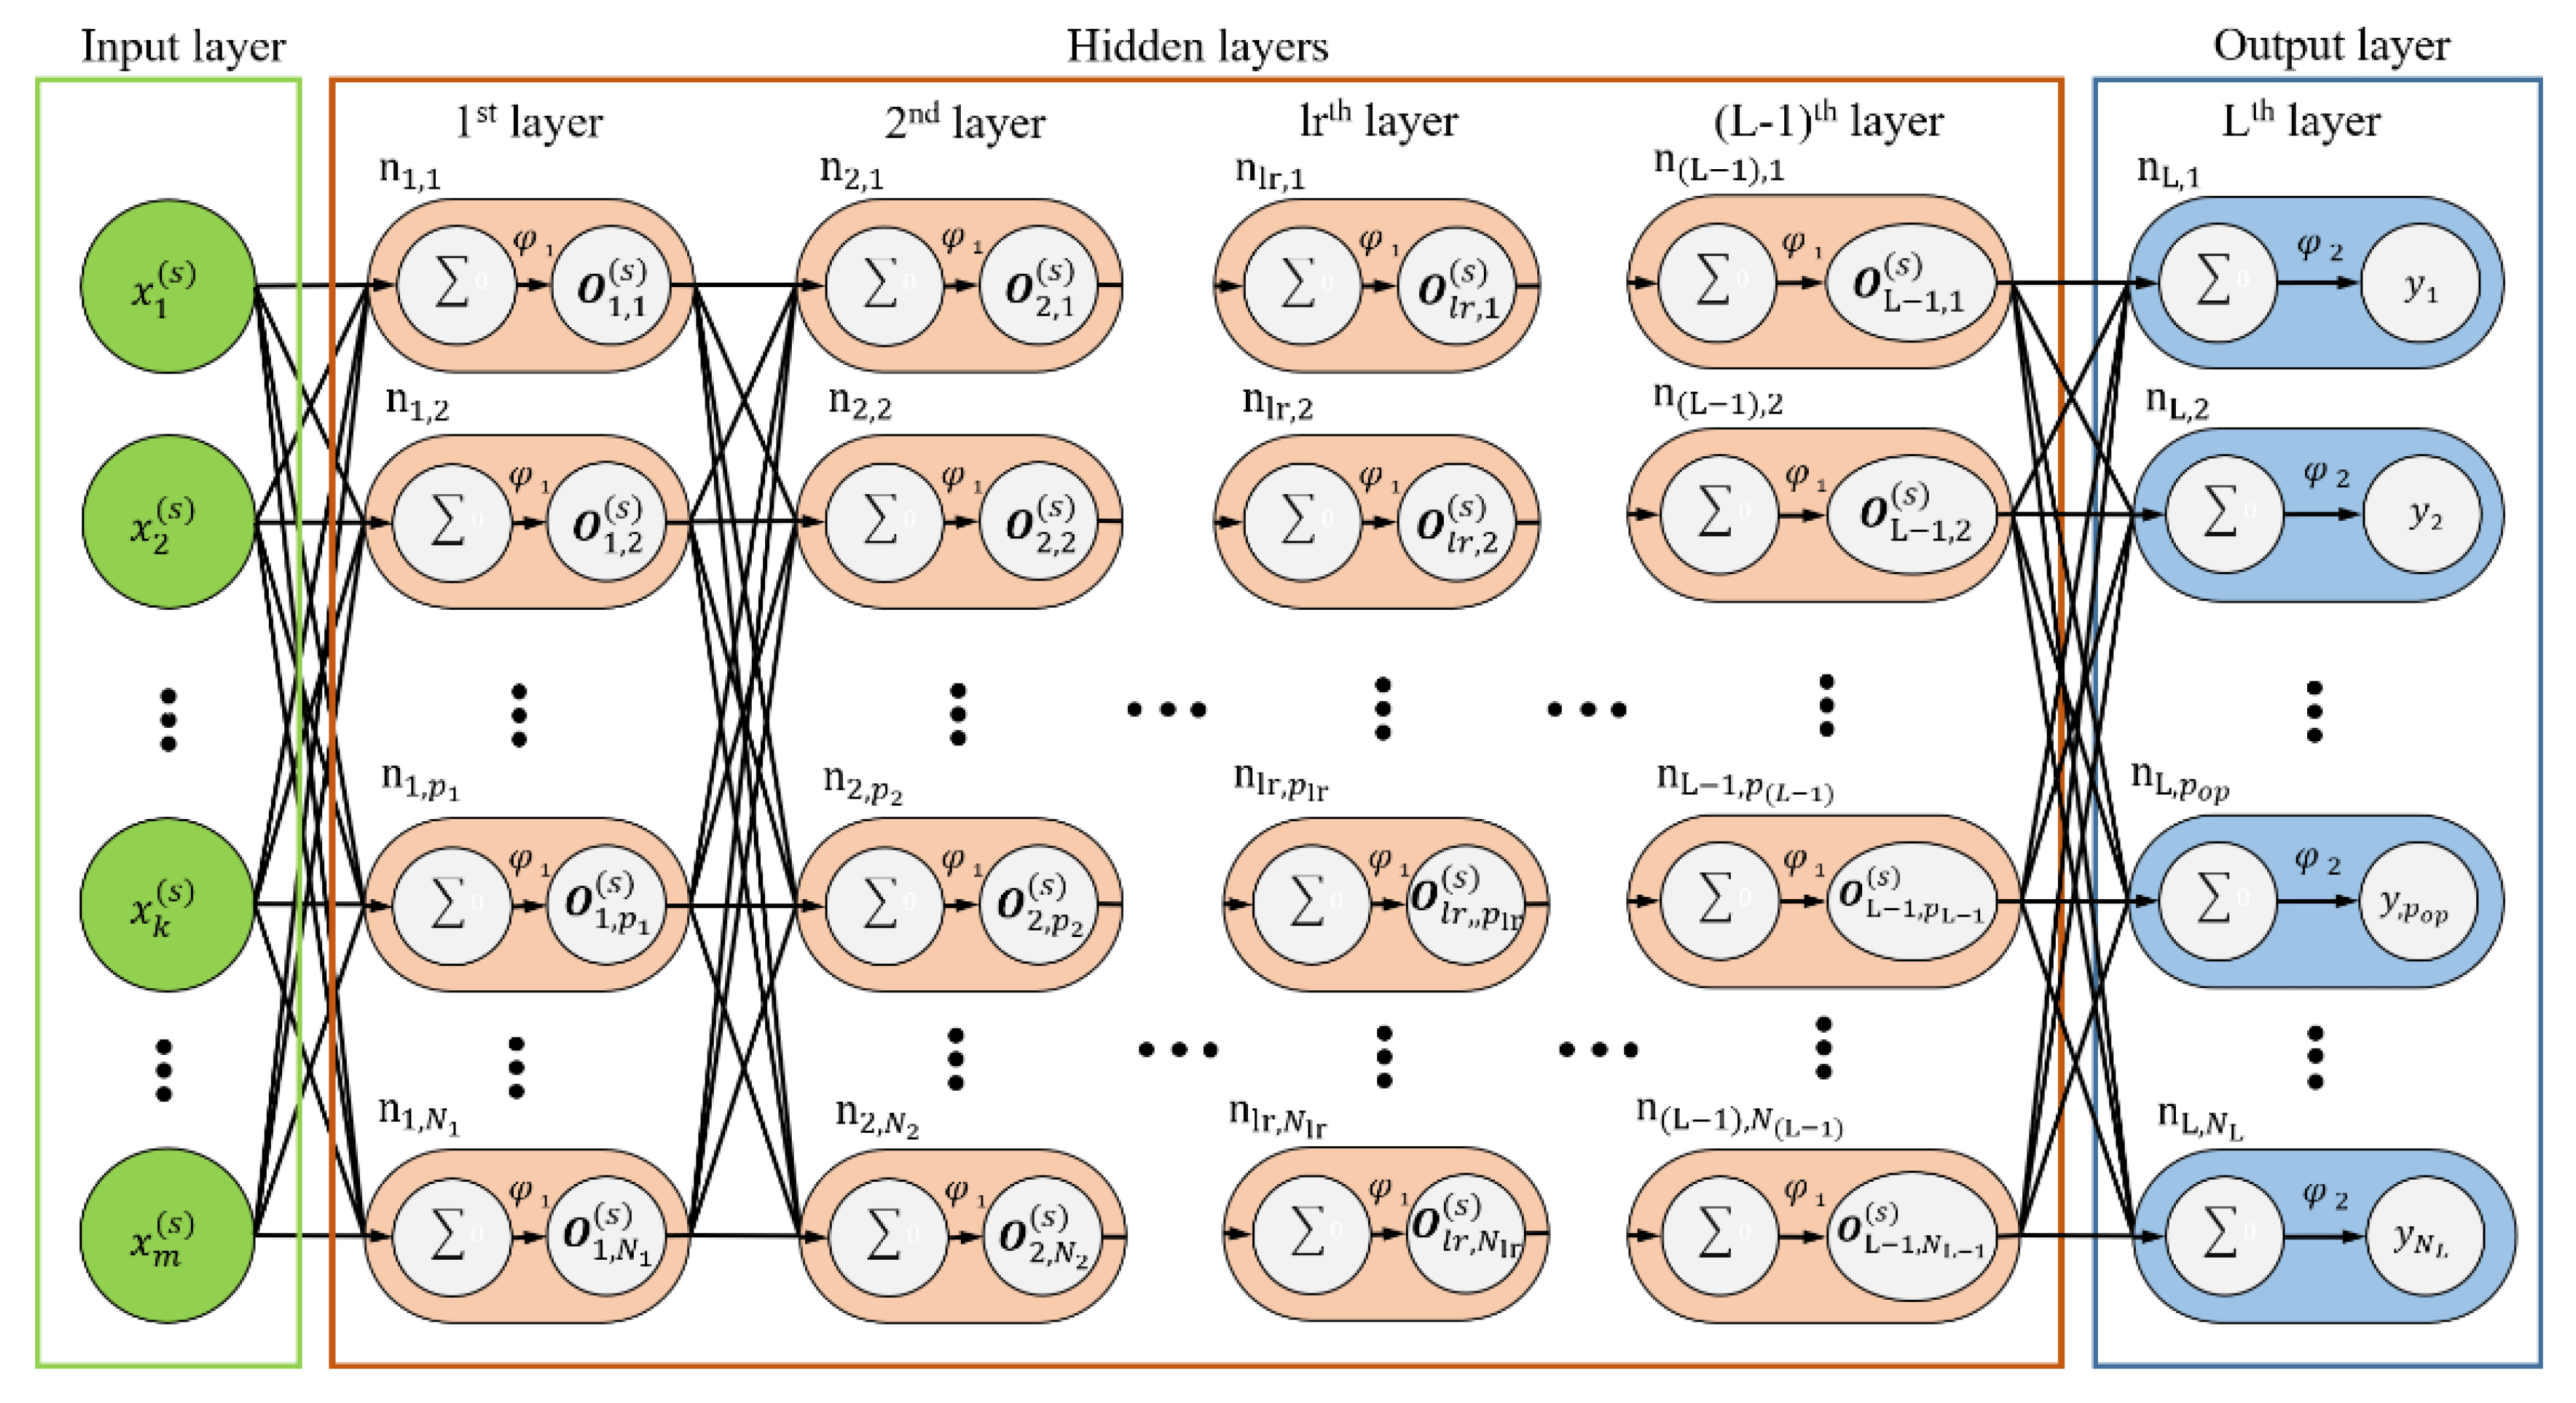
\includegraphics[width=\linewidth]{Figure_algorithm/mlp.png}
    \caption{Structure of the MLP model \cite{mlp_image}}
    \label{fig_mlp}
  \end{minipage}
\end{figure}

The formula to calculate the input values of a layer (except the input layer):
\[ z^{(l)} = W^{(l) T}\alpha^{(l-1)} + b^{(l)} \]
Where:
    \begin{itemize}
        \item $z^{(l)}$ is a matrix containing the input values for each neuron in layer (l)
        \item $W^{(l)}$ is a matrix containing the connection weights between neurons in layer (l-1) and neurons in layer (l)
        \item $\alpha^{(l-1)}$ is a matrix containing the output values of layer (l-1) and serves as the input for layer (l). For the layer immediately following the input layer, it will be replaced by matrix X
        \item $b^{(l)}$ is a matrix containing the threshold values for each neuron in layer (l)
    \end{itemize}
        
When the input value exceeds the threshold, meaning the neuron's z value is greater than 0, the neuron will produce an output value. The formula to calculate the output of a layer (except the input layer):
\[ \alpha^{(l)} = f(z^{(l)}) \]
Where:
    \begin{itemize}
        \item $\alpha^{(l)}$ is a matrix containing the output values of each neuron belonging to layer l
        \item  $f()$ is an activation function, such as the sigmoid, ReLU, or tanh function
    \end{itemize}\\
    
\section{Result}
\subsection{Evaluation Methods}
\textbf{Mean Percentage Absolute Error} (MAPE): is the average percentage error in a set of predicted values.\\
\[MAPE=\frac{100\%}{n}  \sum_{i=1}^{n} |\frac{y_i-\hat{y_i}}{y_i}|\]\\
\textbf{Root Mean Squared Error} (RMSE): is the square root of the average value of squared error in a set of predicted values.\\
\[RMSE=\sqrt{\frac{1}{n} \sum_{i=1}^{n}(\hat{y_i}-y_i )^2}\]\\
\textbf{Mean Absolute Error} (MAE): is a measure of the average difference between predicted values and actual values in a dataset.\\
\[MAE = \frac{1}{n} \sum_{i=1}^{n} |y_i - \hat{y_i}| \]
Where: \\
	\indent\textbullet\ \(n\) is the number of observations in the dataset.\\
	\indent\textbullet\ \(y_i\)  is the true value.\\
	\indent\textbullet\ \(\hat{y_i}\) is the predicted value.
        \cite{sefidian_guide}
\subsection{EUR-VND Dataset} 
\begin{table}[H]
    \centering
    \begin{tabular}{|c|c|c|c|c|}
         \hline
         \multicolumn{5}{|c|}{\textbf{EUR-VND Dataset's Evaluation}}\\
         \hline
         \centering Model & Train:Test & RMSE & MAPE (\%) & MAE\\
         \hline
         \multirow{2}{*}{LR} &\textbf{7:3} &\textbf{1261.17} &\textbf{3.632} &\textbf{993.698} \\ &\ 8:2 &\ 1447.716 &\ 4.61 &\ 1267.462 \\&\ 9:1 &\ 1604.473 &\ 5.581 &\ 1549.852 \\
         \hline
         \multirow{2}{*}{ARIMA} & 7:3 & 1830.875 & 6.224 & 1687.944 \\ & 8:2 & 987.512 & 2.998 & 825.492 \\ & \textbf{9:1} & \textbf{610.009} & \textbf{1.789} &\ \textbf{499.686} \\
         \hline
         \multirow{2}{*}{ETS} & 7:3 & 1631.753 & 5.547 & 1504.453 \\ & 8:2 & 532.582&1.5499&426.105 \\& \textbf{9:1} & \textbf{236.536} & \textbf{0.696} & \textbf{192.593} \\
         \hline
         \multirow{2}{*}{Stacking} &\ 7:3 &\ 1443.383 &\ 4.991 &\ 1323.673 \\ &\ 8:2 &\textbf{698.075} &\textbf{2.066} &\textbf{553.825}\\&\ 9:1 &\ 822.191 &\ 2.511 &\ 700.179 \\
         \hline
         \multirow{2}{*}{RNN} & 7:3 & 93.655 & 0.252 & 67.515 \\ & 8:2 & 92.962 & 0.254 & 69.081 \\ & \textbf{9:1} & \textbf{81.738} & \textbf{0.205} &\ \textbf{56.667} \\
         \hline
         \multirow{2}{*}{GRU} & 7:3 & 95.492 & 0.259 & 69.448 \\ & 8:2 & 93.5 & 0.253 & 68.955 \\ & \textbf{9:1} & \textbf{82.348} & \textbf{0.204} &\ \textbf{56.4306} \\
         \hline
         \multirow{2}{*}{LSTM} &\ 7:3 &\ 101.108 &0.287 &77.325\\ &\ 8:2 &\ 127.054&\ 0.367 &\ 100.78 \\&\textbf{9:1}&\textbf{95.397} &\textbf{0.26} &\textbf{72.617} \\
         \hline
         \multirow{2}{*}{MLP} & 7:3 & 101.67 & 0.276 & 74.146 \\ & 8:2 & 90.746 & 0.243 & 65.98 \\ & \textbf{9:1} & \textbf{84.833} & \textbf{0.214} &\ \textbf{59.271} \\
         \hline
    \end{tabular}
    \caption{EUR-VND Dataset's Evaluation}
    \label{vcbresult}
\end{table}

\begin{figure}[H]
  \centering
  \begin{minipage}{0.8\linewidth}
    \centering
    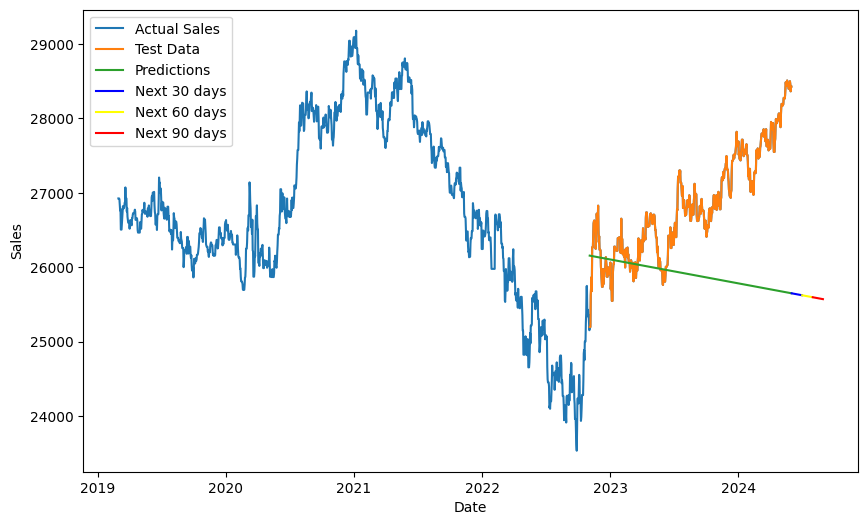
\includegraphics[width=\linewidth]{LR/linear_eur73.png}
    \caption{Linear Regression model's result with 7:3 splitting proportion}
    \label{fig10}
  \end{minipage}
\end{figure}
\begin{figure}[H]
  \centering
  \begin{minipage}{0.8\linewidth}
    \centering
    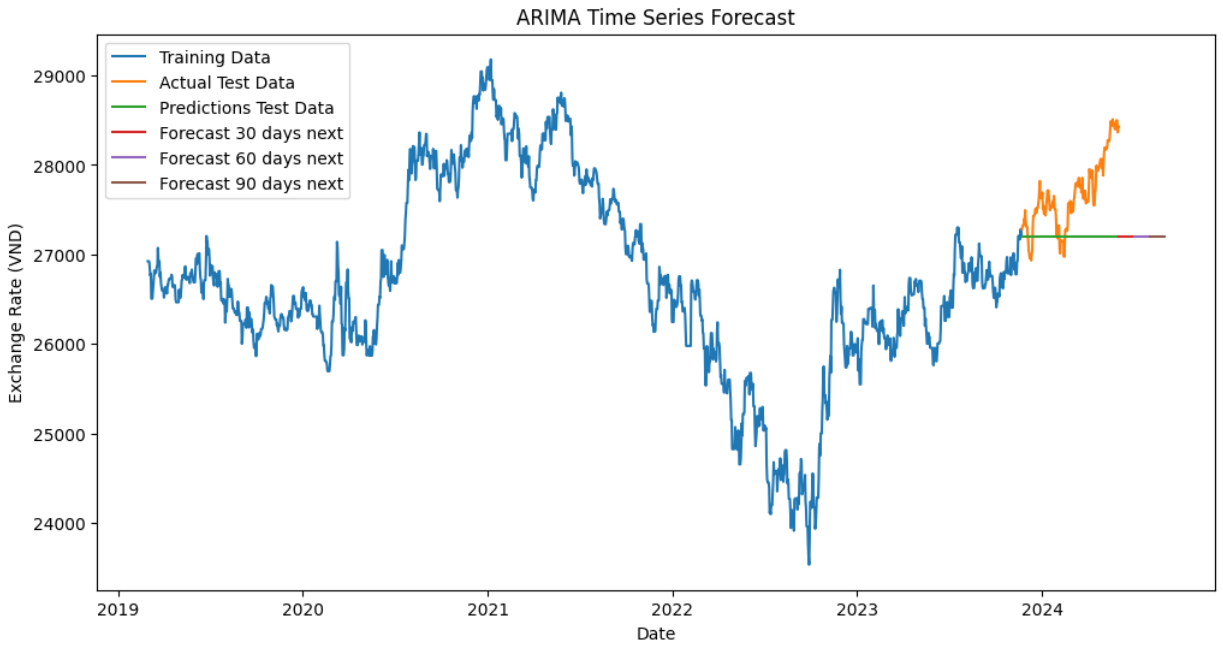
\includegraphics[width=\linewidth]{ARIMA/arima_eur_91.png}
    \caption{ARIMA model's result with 9:1 splitting proportion}
    \label{fig11}
  \end{minipage}
\end{figure}
\begin{figure}[H]
  \centering
  \begin{minipage}{0.8\linewidth}
    \centering
    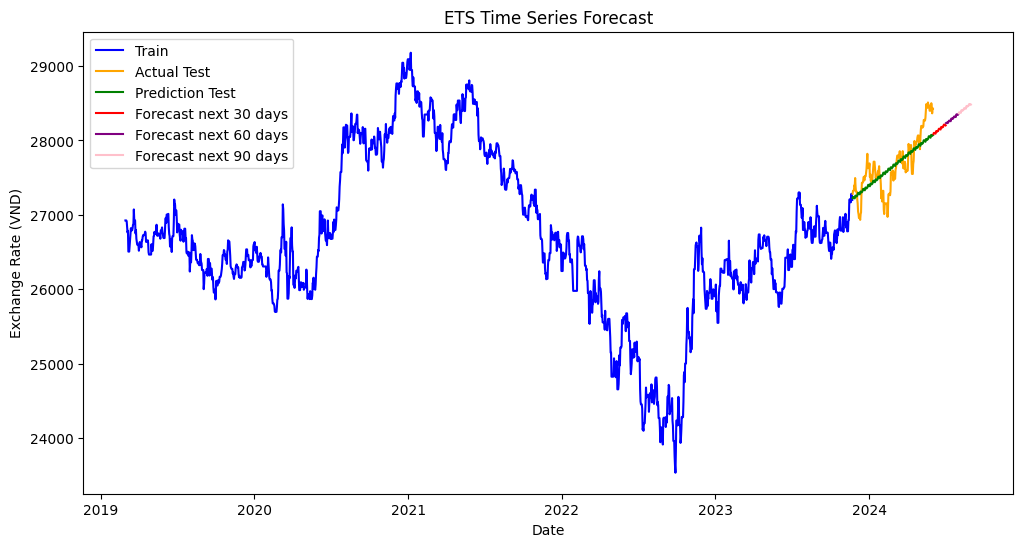
\includegraphics[width=\linewidth]{ETS/ETS_eur_91.png}
    \caption{ETS model's result with 9:1 splitting proportion}
    \label{fig12}
  \end{minipage}
\end{figure}
\begin{figure}[H]
  \centering
  \begin{minipage}{0.8\linewidth}
    \centering
    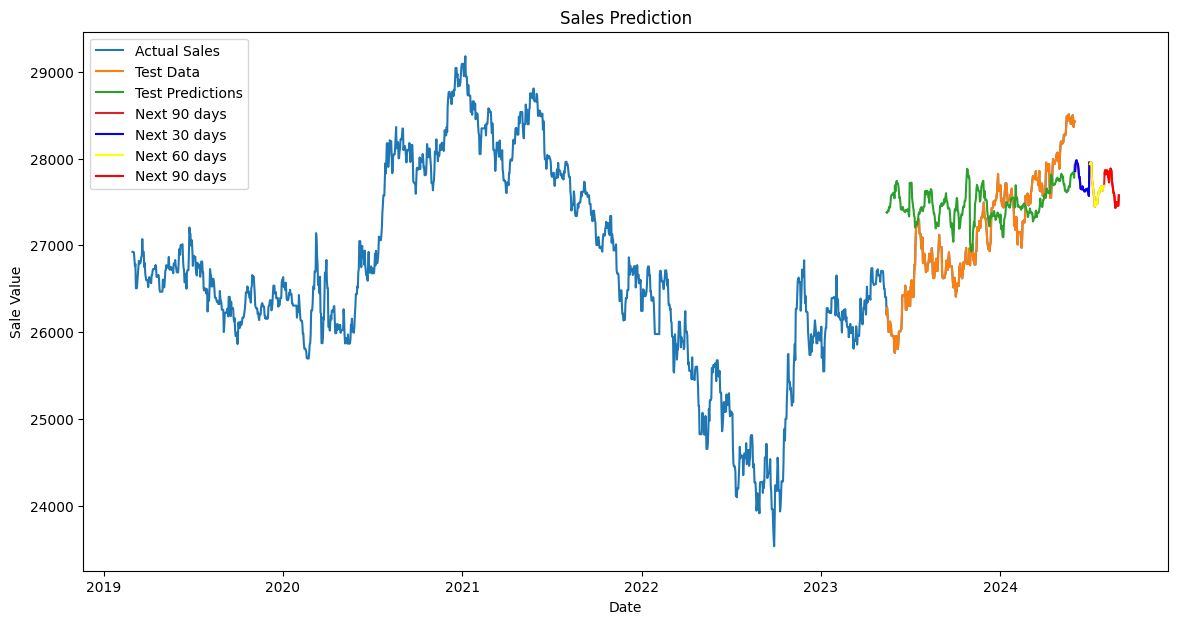
\includegraphics[width=\linewidth]{Stacking/stmodel_eur82.png}
    \caption{Stacking model's result with 8:2 splitting proportion}
    \label{fig13}
  \end{minipage}
\end{figure}
\begin{figure}[H]
  \centering
  \begin{minipage}{0.8\linewidth}
    \centering
    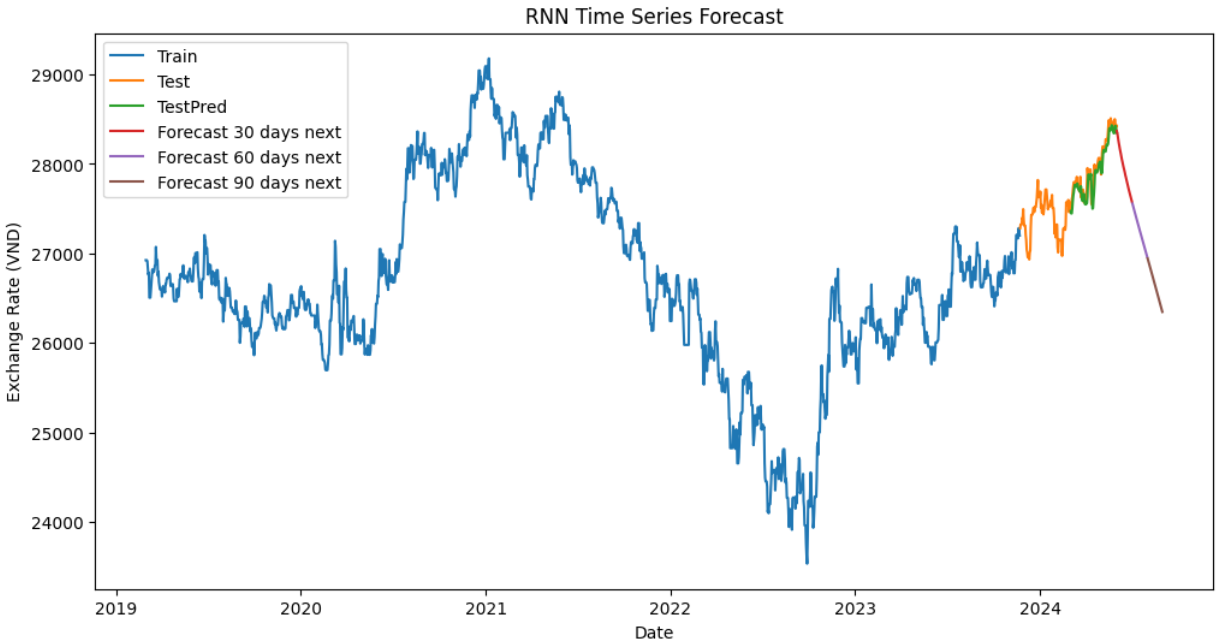
\includegraphics[width=\linewidth]{RNN/rnn_eur_91.png}
    \caption{RNN model's result with 9:1 splitting proportion}
    \label{fig14}
  \end{minipage}
\end{figure}
\begin{figure}[H]
  \centering
  \begin{minipage}{0.8\linewidth}
    \centering
    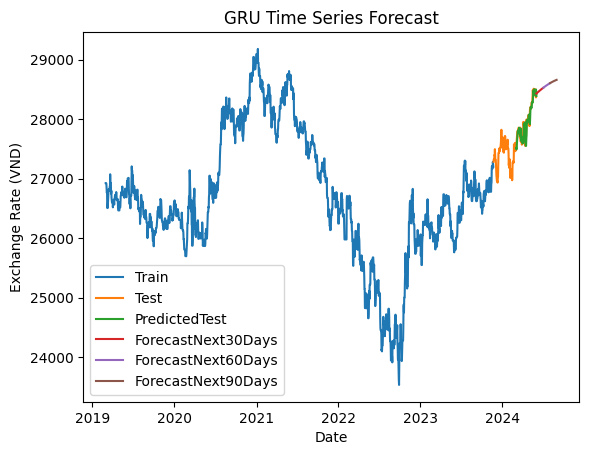
\includegraphics[width=\linewidth]{GRU/GRU_eur_91.png}
    \caption{GRU model's result with 9:1 splitting proportion}
    \label{fig15}
  \end{minipage}
\end{figure}
\begin{figure}[H]
  \centering
  \begin{minipage}{0.8\linewidth}
    \centering
    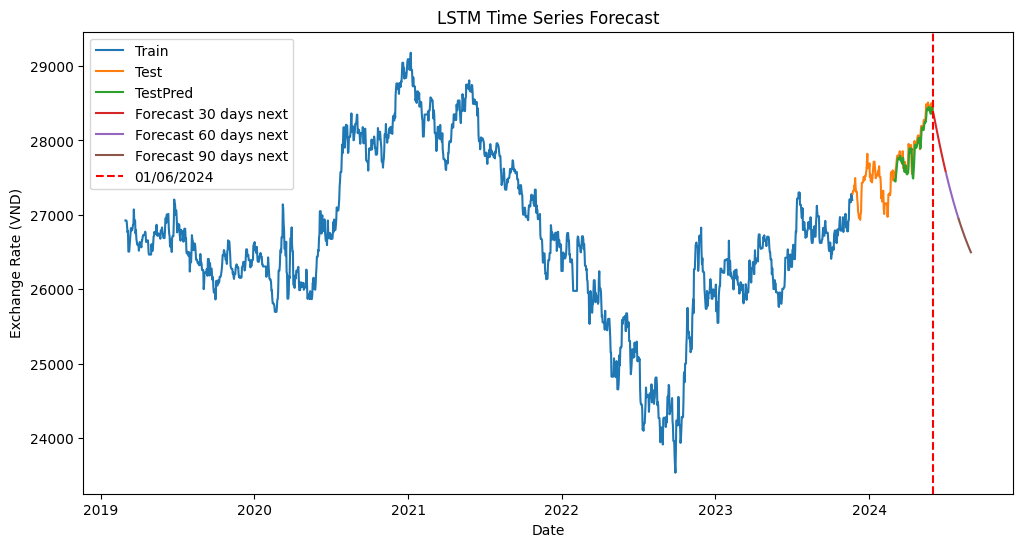
\includegraphics[width=\linewidth]{LSTM/lstm_eur91.png}
    \caption{LSTM model's result with 9:1 splitting proportion}
    \label{fig16}
  \end{minipage}
\end{figure}
\begin{figure}[H]
  \centering
  \begin{minipage}{0.8\linewidth}
    \centering
    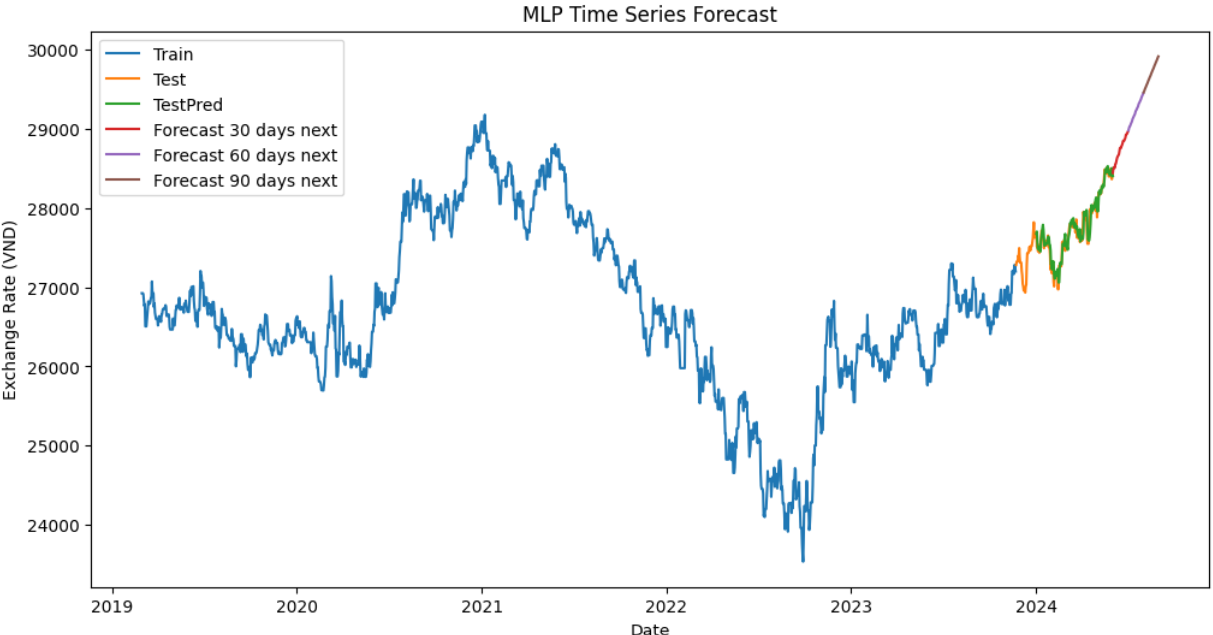
\includegraphics[width=\linewidth]{MLP/mlp_eur_91.png}
    \caption{MLP model's result with 9:1 splitting proportion}
    \label{fig17}
  \end{minipage}
\end{figure}

\subsection{GBP-VND dataset} 
\begin{table}[H]
    \centering
    \begin{tabular}{|c|c|c|c|c|}
         \hline
         \multicolumn{5}{|c|}{\textbf{GBP-VND Dataset's Evaluation}}\\
         \hline
         \centering Model & Train:Test & RMSE & MAPE (\%) & MAE\\
         \hline
         \multirow{2}{*}{LR} &\textbf{7:3} &\textbf{1112.325} &\textbf{2.996} &\textbf{926.064} \\ &\ 8:2 &\ 1545.954	&\ 4.135 &\ 1315.139 \\&\ 9:1 &\ 1851.111 &\ 5.532 &\ 1779.392 \\
         \hline
         \multirow{2}{*}{ARIMA} &\ 7:3 &\ 2266.597 &\ 6.304 &\ 1974.25 \\ &\ 8:2 &\ 1610.114 &\ 4.373 &\ 1390.125 \\&\ \textbf{9:1} &\ \textbf{1112.536} &\ \textbf{3.071} &\ \textbf{991.12} \\
         \hline
         \multirow{2}{*}{ETS} & 7:3 & 1751.462&5.0491&1569.855 \\ & 8:2 & 1081.92&3.0195&952.128 \\& \textbf{9:1} & \textbf{314.804} & \textbf{0.817} & \textbf{261.519} \\
         \hline
         \multirow{2}{*}{Stacking Model} &\ 7:3 &\ 1373.337 &\ 	3.719 &\ 	1160.102\\ & \textbf{8:2} &\textbf{967.166	} &\textbf{	2.466} &\textbf{780.687}\\&\ 9:1 &\ 1416.977	&3.957	&1276.006 \\
         \hline
         \multirow{2}{*}{RNN} & 7:3 & 125.438 & 0.297 & 90.847 \\ & 8:2 & 122.789 & 0.294 & 92.395 \\ & \textbf{9:1} & \textbf{105.797} & \textbf{0.234} &\ \textbf{75.146} \\
         \hline
         \multirow{2}{*}{GRU} & 7:3 & 124.999 & 0.286 & 87.592 \\ & 8:2 & 128.489 & 0.3153 & 99.099 \\ & \textbf{9:1} & \textbf{106.643} & \textbf{0.232} &\ \textbf{74.63} \\
         \hline
         \multirow{2}{*}{LSTM} &\ 7:3 &147.362&	0.374	&115.568 \\ &\ 8:2 &122.03&	0.293&	92.348 \\&\textbf{9:1}&\textbf{121.924		} &\textbf{0.291} &\textbf{94.226} \\
         \hline
         \multirow{2}{*}{MLP} & 7:3 & 154.242 & 0.397 & 122.14 \\ & 8:2 & 128.465 & 0.311 & 97.161 \\ & \textbf{9:1} & \textbf{116.821} & \textbf{0.277} &\ \textbf{88.954} \\
         \hline
    \end{tabular}
    \caption{GBP-VND Dataset's Evaluation}
    \label{mbbresult}
\end{table}

\begin{figure}[H]
  \centering
  \begin{minipage}{0.8\linewidth}
    \centering
    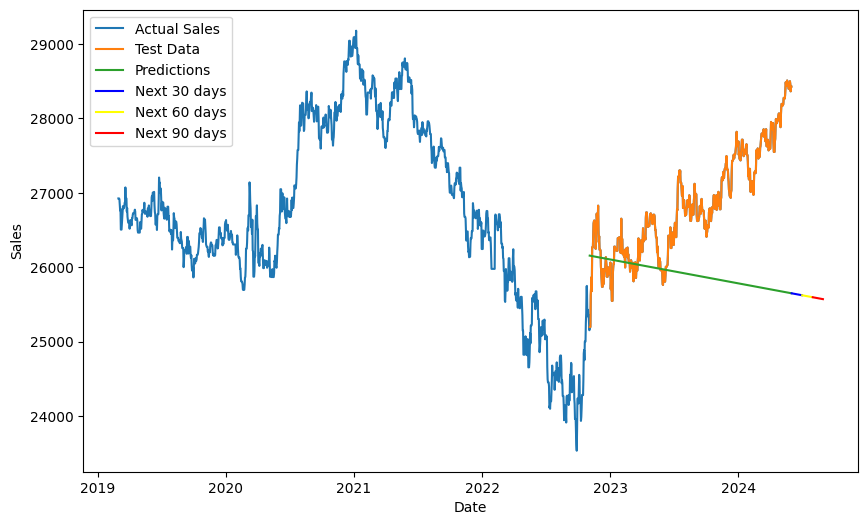
\includegraphics[width=\linewidth]{LR/linear_gbp73.png}
    \caption{Linear Regression model's result with 7:3 splitting proportion}
    \label{fig18}
  \end{minipage}
\end{figure}
\begin{figure}[H]
  \centering
  \begin{minipage}{0.8\linewidth}
    \centering
    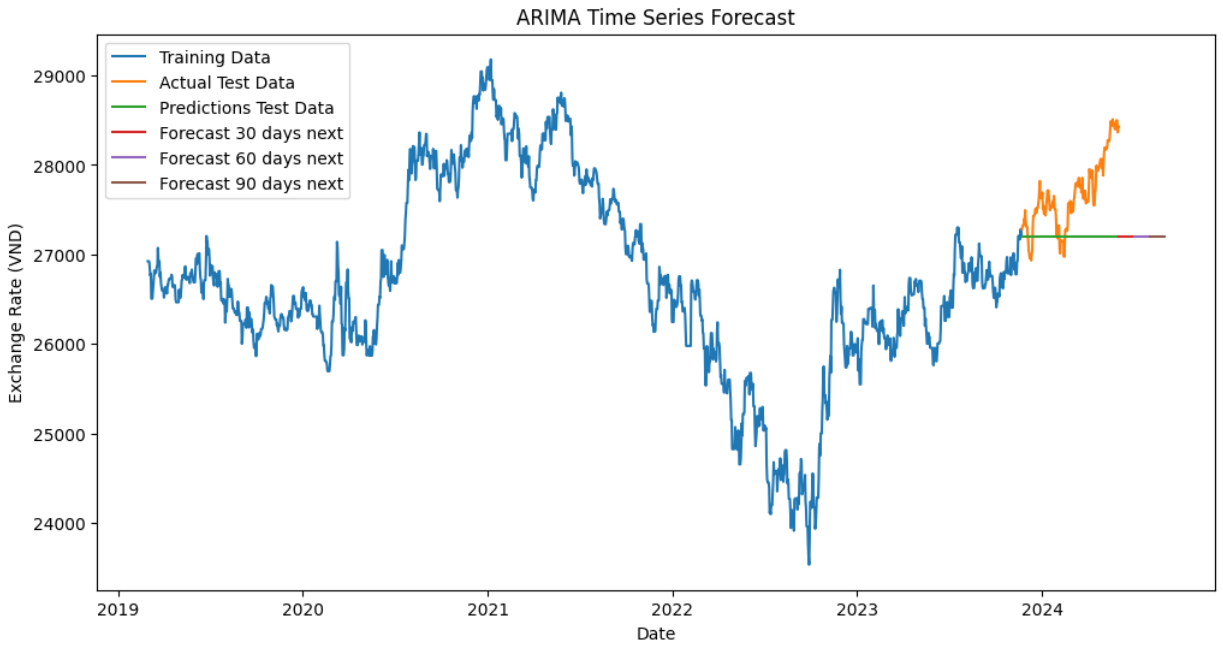
\includegraphics[width=\linewidth]{ARIMA/arima_eur_91.png}
    \caption{ARIMA model's result with 9:1 splitting proportion}
    \label{fig19}
  \end{minipage}
\end{figure}
\begin{figure}[H]
  \centering
  \begin{minipage}{0.8\linewidth}
    \centering
    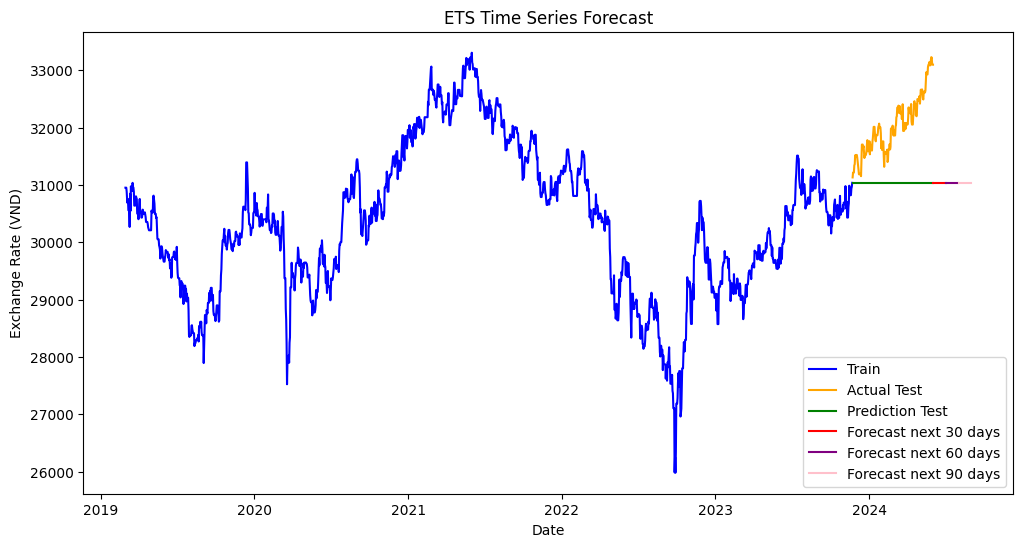
\includegraphics[width=\linewidth]{ETS/ETS_gbp_91.png}
    \caption{ETS model's result with 9:1 splitting proportion}
    \label{fig20}
  \end{minipage}
\end{figure}
\begin{figure}[H]
  \centering
  \begin{minipage}{0.8\linewidth}
    \centering
    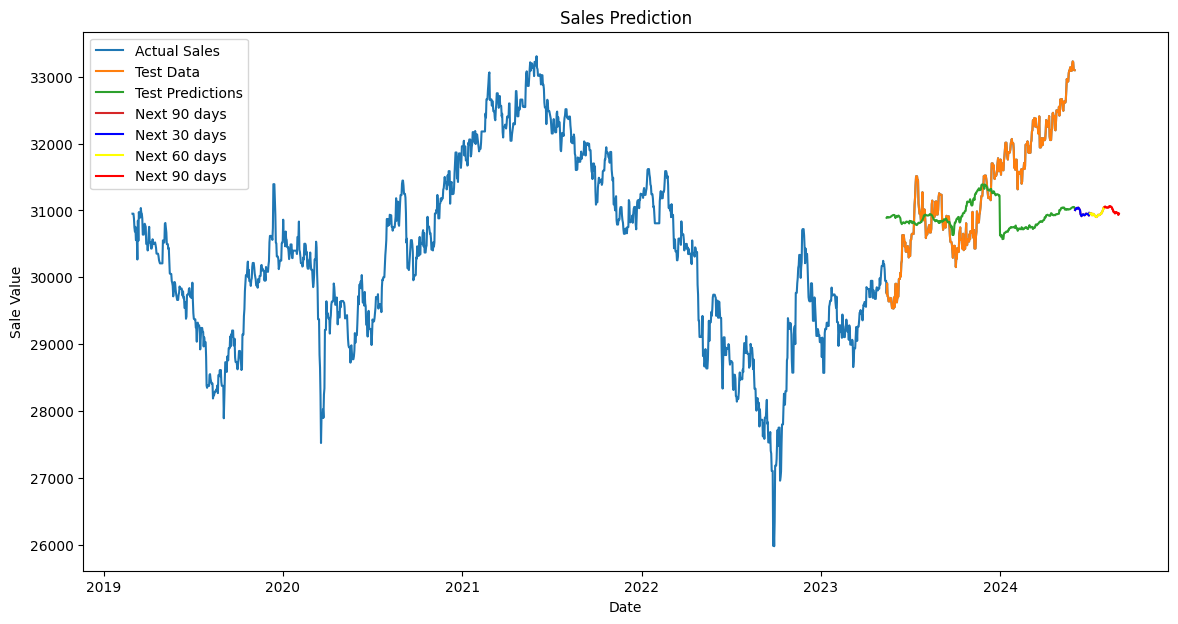
\includegraphics[width=\linewidth]{Stacking/stmodel_gbp82.png}
    \caption{Stacking model's result with 8:2 splitting proportion}
    \label{fig21}
  \end{minipage}
\end{figure}
\begin{figure}[H]
  \centering
  \begin{minipage}{0.8\linewidth}
    \centering
    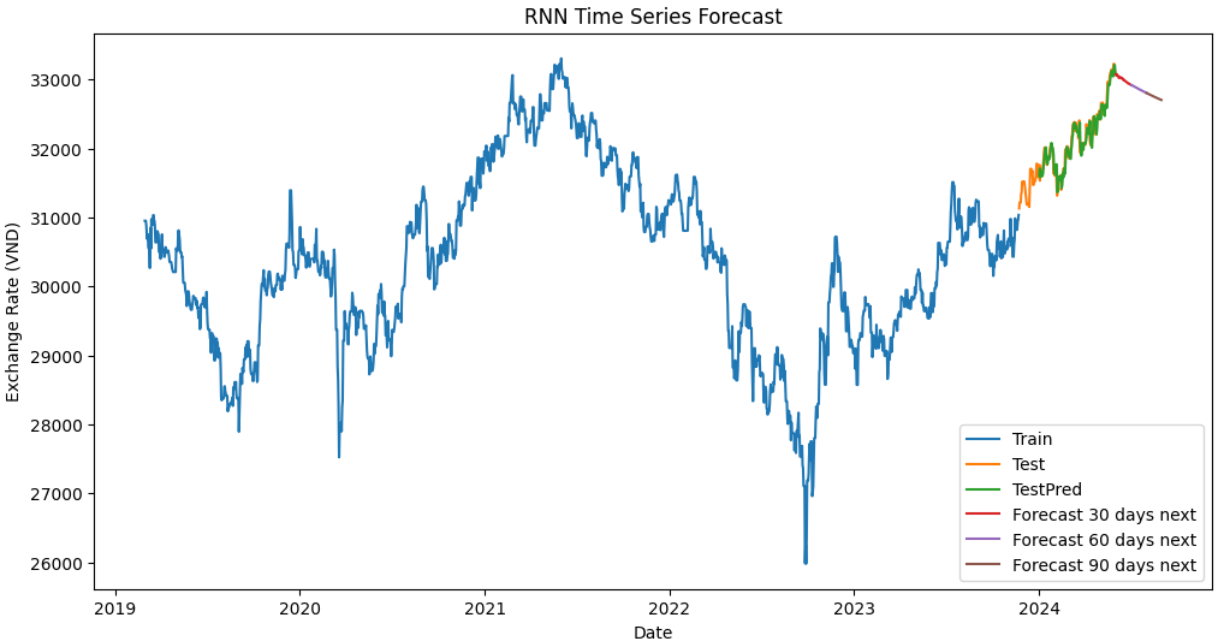
\includegraphics[width=\linewidth]{RNN/rnn_gbp_91.png}
    \caption{RNN model's result with 9:1 splitting proportion}
    \label{fig22}
  \end{minipage}
\end{figure}
\begin{figure}[H]
  \centering
  \begin{minipage}{0.8\linewidth}
    \centering
    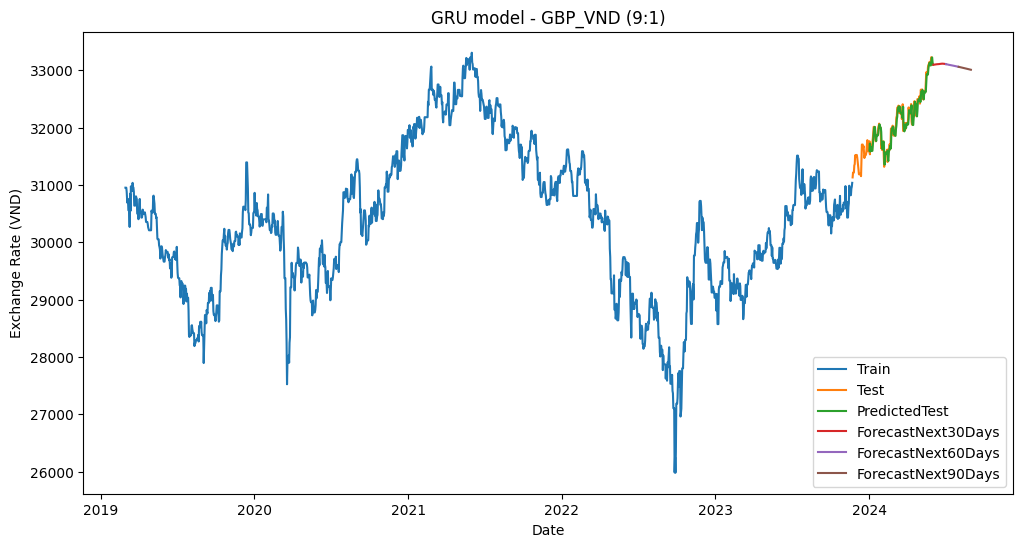
\includegraphics[width=\linewidth]{GRU/GRU_gbp_91.png}
    \caption{GRU model's result with 9:1 splitting proportion}
    \label{fig23}
  \end{minipage}
\end{figure}
\begin{figure}[H]
  \centering
  \begin{minipage}{0.8\linewidth}
    \centering
    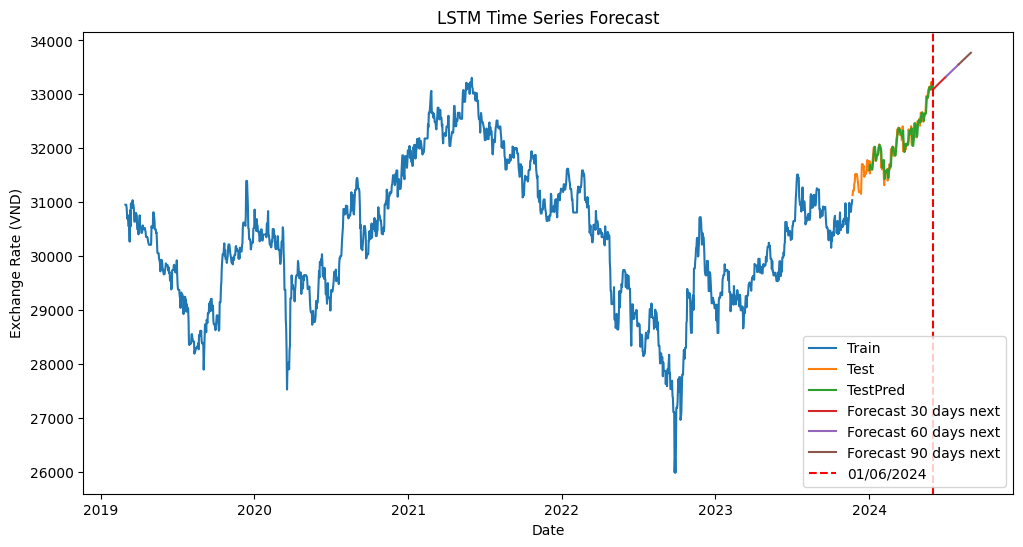
\includegraphics[width=\linewidth]{LSTM/lstm_gbp91.png}
    \caption{LSTM model's result with 9:1 splitting proportion}
    \label{fig24}
  \end{minipage}
\end{figure}
\begin{figure}[H]
  \centering
  \begin{minipage}{0.8\linewidth}
    \centering
    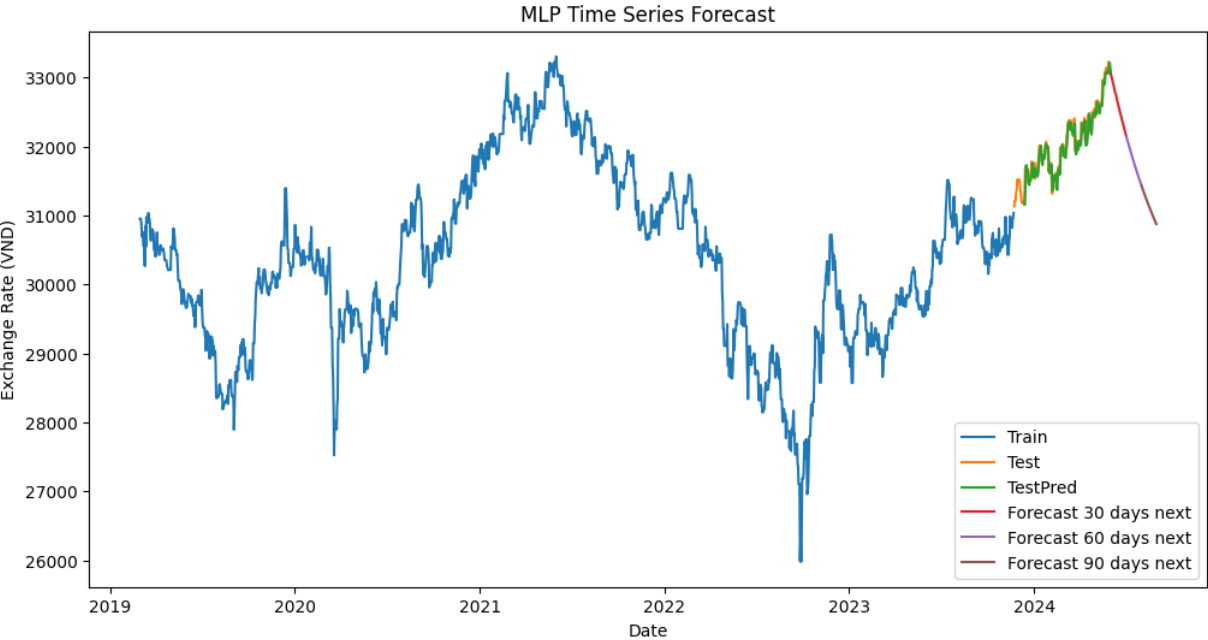
\includegraphics[width=\linewidth]{MLP/mlp_gbp_91.png}
    \caption{MLP model's result with 9:1 splitting proportion}
    \label{fig25}
  \end{minipage}
\end{figure}

\subsection{JPY-VND dataset} 
\begin{table}[H]
    \centering
    \begin{tabular}{|c|c|c|c|c|}
         \hline
         \centering Model & Train:Test & RMSE & MAPE (\%) & MAE\\
         \hline
         \multirow{2}{*}{LR} & 7:3 & 8.201 & 4.226 & 7.296 \\ & 8:2 & 6.661	& 3.349	& 5.703 \\&\textbf{9:1} &\textbf{2.559} &\textbf{1.207} &\textbf{2.078} \\
         \hline
         \multirow{2}{*}{ARIMA} & 7:3 & 10.529 & 5.592 & 9.836 \\ & 8:2 & 9.014 & 5.089 & 8.656 \\& \textbf{9:1} & \textbf{5.955} & \textbf{3.239} & \textbf{5.565} \\
         \hline
         \multirow{2}{*}{ETS} & 7:3 & 10.054&5.298&9.326 \\ & \textbf{8:2} &\textbf{5.459}&\textbf{2.853} &\textbf{4.852} \\& 9:1 &5.883&3.194&5.488 \\
         \hline
         \multirow{2}{*}{Stacking Model} &\ 7:3 &\ 27.438	&13.326	&23.19 \\&\ 8:2 &13.681	&7.595&	12.946\\ & \textbf{9:1} &\textbf{6.886} &\textbf{3.577} &\textbf{6.127}\\
         \hline
         \multirow{2}{*}{RNN} & 7:3 & 1.119 & 0.444 & 0.779 \\ &\textbf{8:2} & \textbf{0.867} & \textbf{0.369} & \textbf{0.629} \\ & 9:1 & 0.87 & 0.396 & 0.675 \\
         \hline
         \multirow{2}{*}{GRU} & 7:3 & 1.044 & 0.408 & 0.714 \\ & 8:2 & 0.86 & 0.355 & 0.607 \\ &\textbf{9:1} & \textbf{0.788} & \textbf{0.332} & \textbf{0.567} \\
         \hline
         \multirow{2}{*}{LSTM} &\ 7:3 &\ 1.267	&0.552	&0.957  \\&\textbf{8:2}&\textbf{0.99} &\textbf{0.43} &\textbf{0.733} \\ &\ 9:1 &\ 1.115&	0.494&	0.839\\
         \hline
         \multirow{2}{*}{MLP} & 7:3 & 1.092 & 0.42 & 0.74 \\ &\textbf{8:2} & \textbf{0.837} & \textbf{0.336} & \textbf{0.575} \\ & 9:1 & 0.887 & 0.366 & 0.627 \\
         \hline
    \end{tabular}
    \caption{JPY-VND Dataset's Evaluation}
    \label{mbbresult}
\end{table}

\begin{figure}[H]
  \centering
  \begin{minipage}{0.8\linewidth}
    \centering
    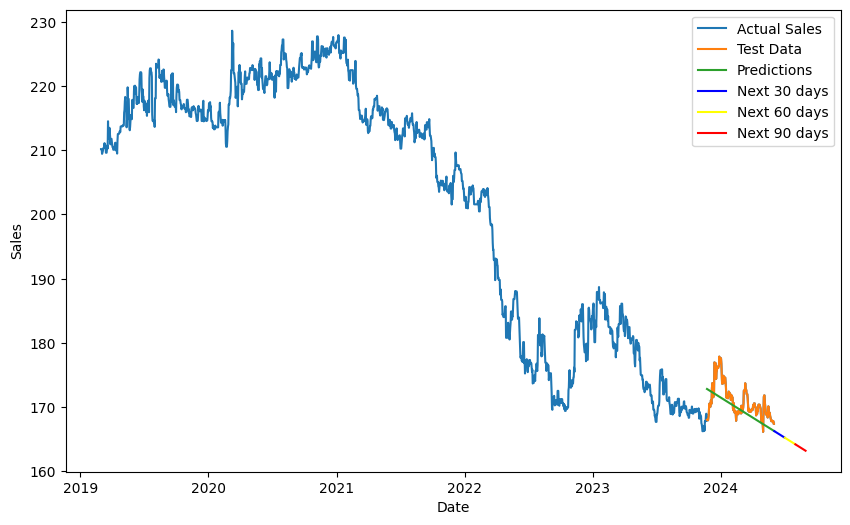
\includegraphics[width=\linewidth]{LR/linear_jpy91.png}
    \caption{Linear Regression model's result with 9:1 splitting proportion}
    \label{fig26}
  \end{minipage}
\end{figure}
\begin{figure}[H]
  \centering
  \begin{minipage}{0.8\linewidth}
    \centering
    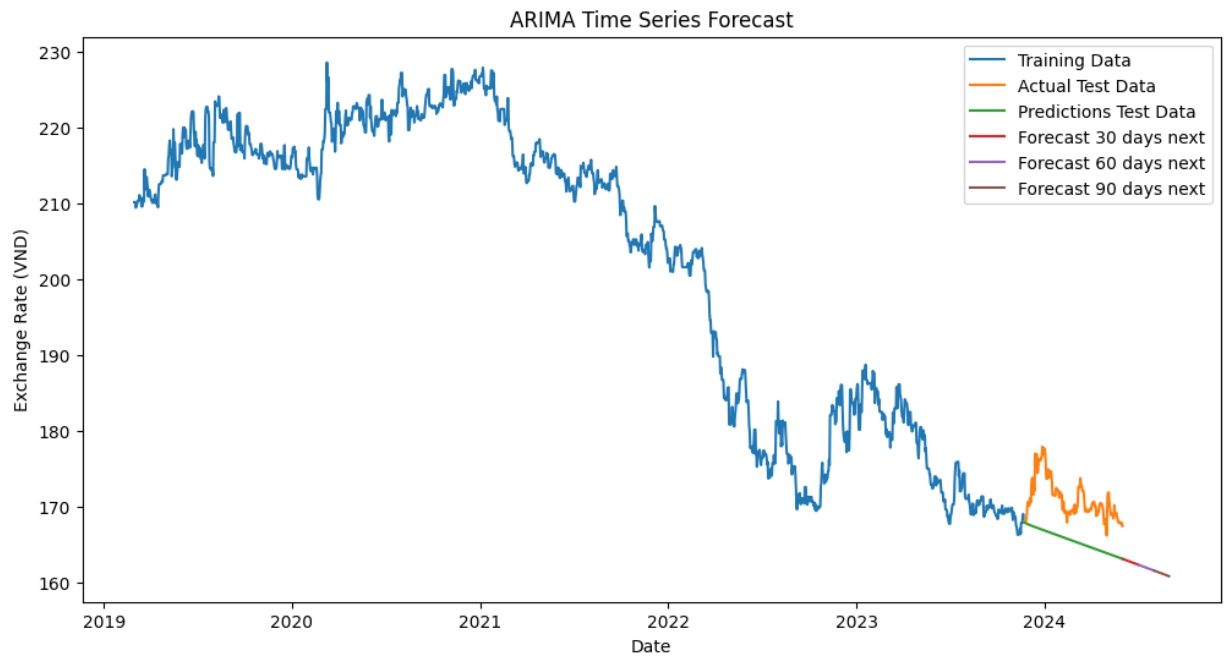
\includegraphics[width=\linewidth]{ARIMA/arima_jpy_91.png}
    \caption{ARIMA model's result with 9:1 splitting proportion}
    \label{fig27}
  \end{minipage}
\end{figure}
\begin{figure}[H]
  \centering
  \begin{minipage}{0.8\linewidth}
    \centering
    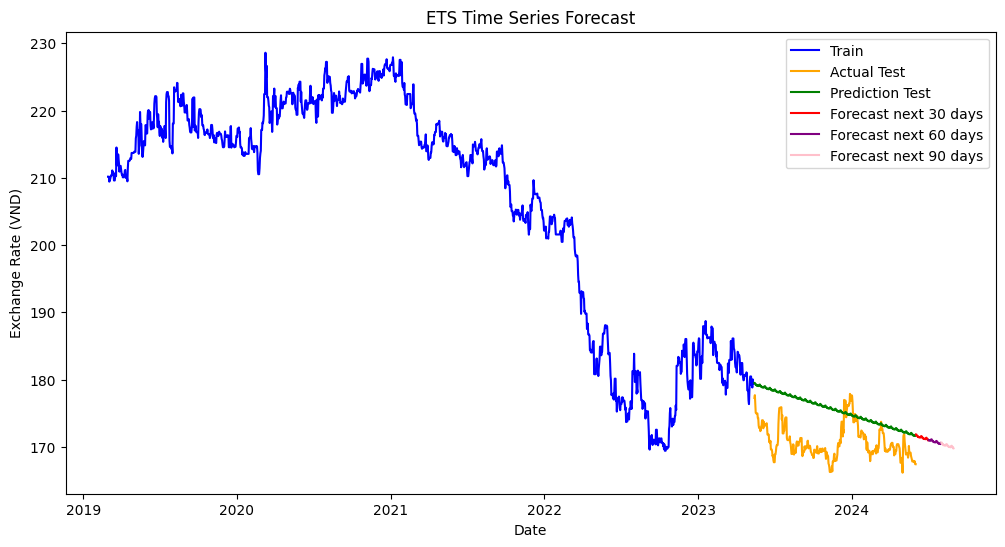
\includegraphics[width=\linewidth]{ETS/ETS_jpy_82.png}
    \caption{ETS model's result with 8:2 splitting proportion}
    \label{fig28}
  \end{minipage}
\end{figure}
\begin{figure}[H]
  \centering
  \begin{minipage}{0.8\linewidth}
    \centering
    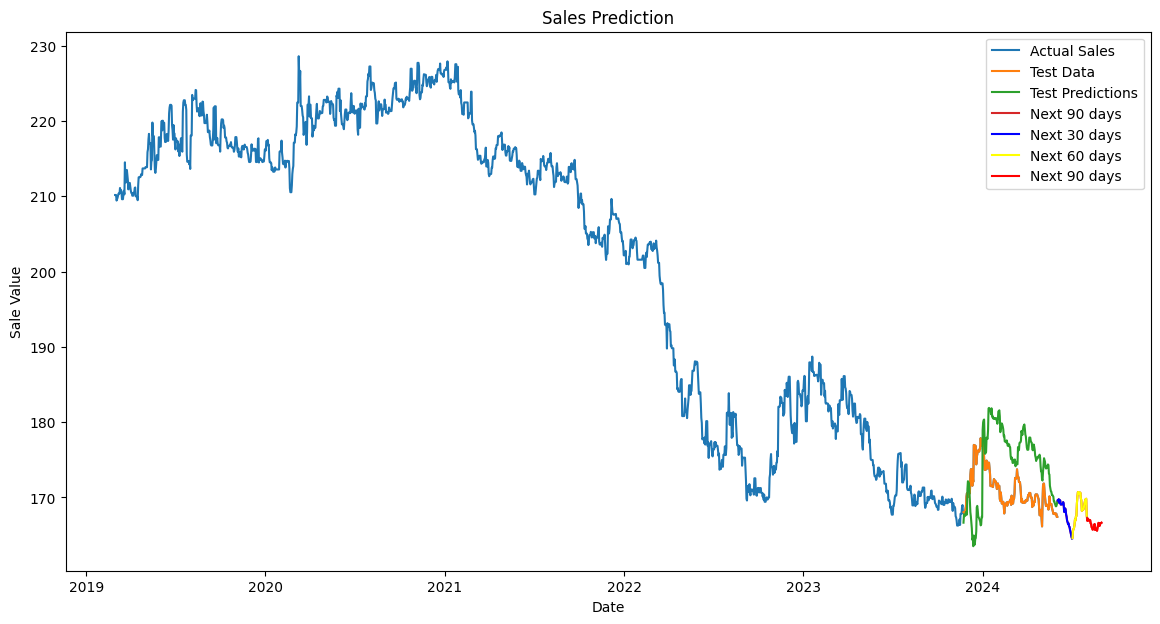
\includegraphics[width=\linewidth]{Stacking/stmodel_jpy91.png}
    \caption{Stacking model's result with 9:1 splitting proportion}
    \label{fig29}
  \end{minipage}
\end{figure}
\begin{figure}[H]
  \centering
  \begin{minipage}{0.8\linewidth}
    \centering
    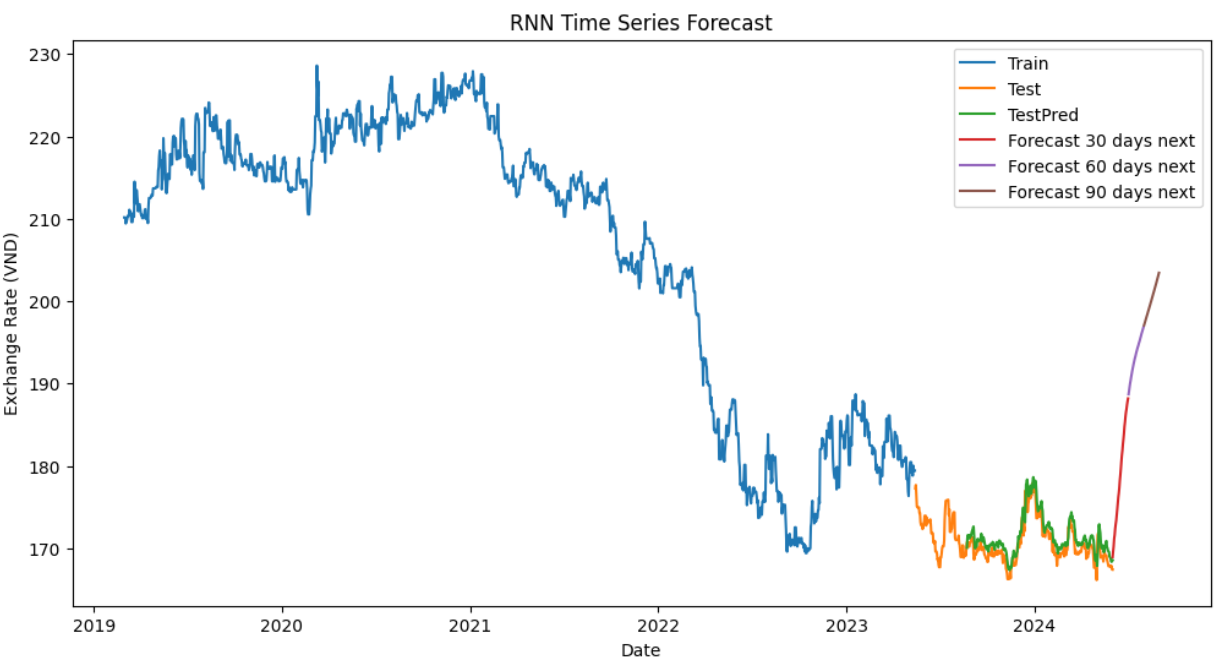
\includegraphics[width=\linewidth]{RNN/rnn_jpy_82.png}
    \caption{RNN model's result with 8:2 splitting proportion}
    \label{fig30}
  \end{minipage}
\end{figure}
\begin{figure}[H]
  \centering
  \begin{minipage}{0.8\linewidth}
    \centering
    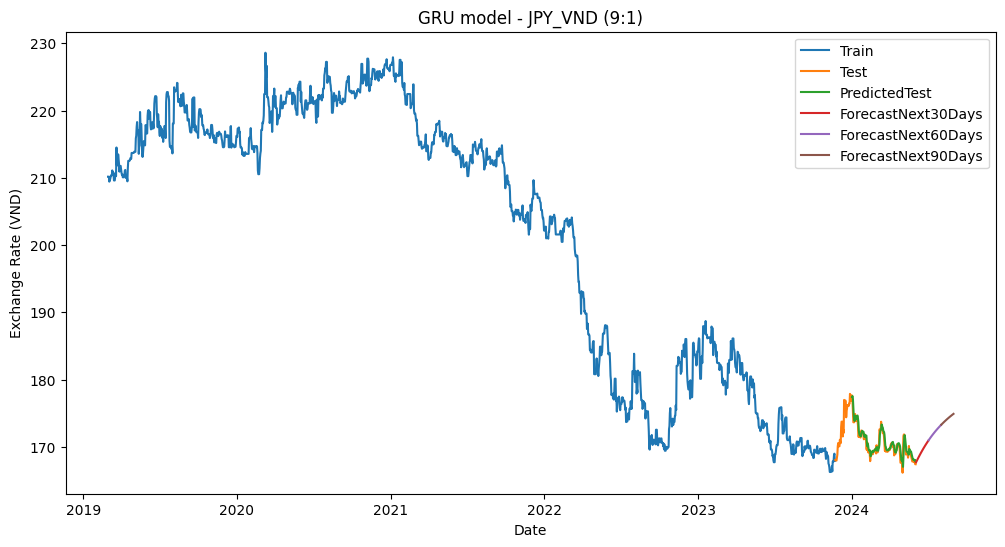
\includegraphics[width=\linewidth]{GRU/GRU_jpy_91.png}
    \caption{GRU model's result with 9:1 splitting proportion}
    \label{fig31}
  \end{minipage}
\end{figure}
\begin{figure}[H]
  \centering
  \begin{minipage}{0.8\linewidth}
    \centering
    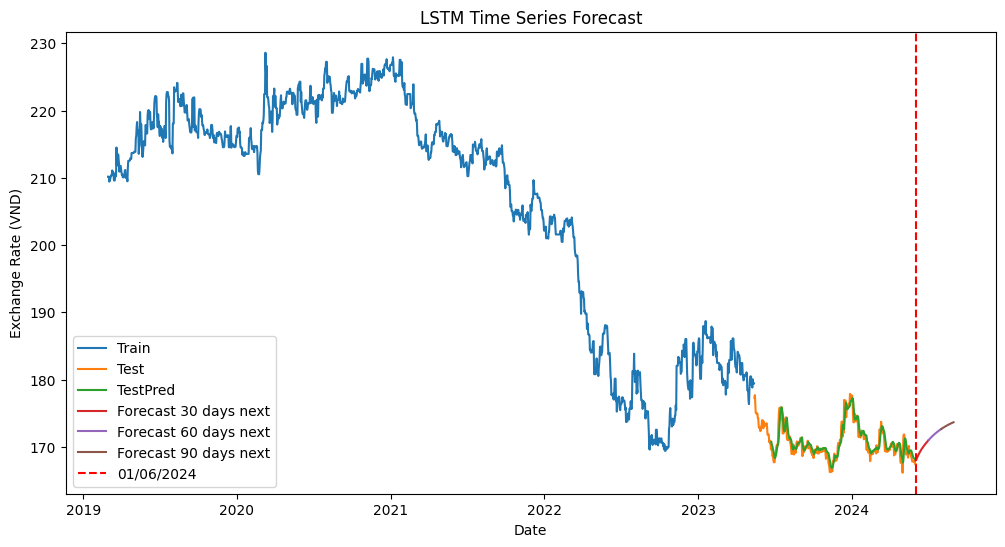
\includegraphics[width=\linewidth]{LSTM/lstm_jpy82.png}
    \caption{LSTM model's result with 8:2 splitting proportion}
    \label{fig32}
  \end{minipage}
\end{figure}
\begin{figure}[H]
  \centering
  \begin{minipage}{0.8\linewidth}
    \centering
    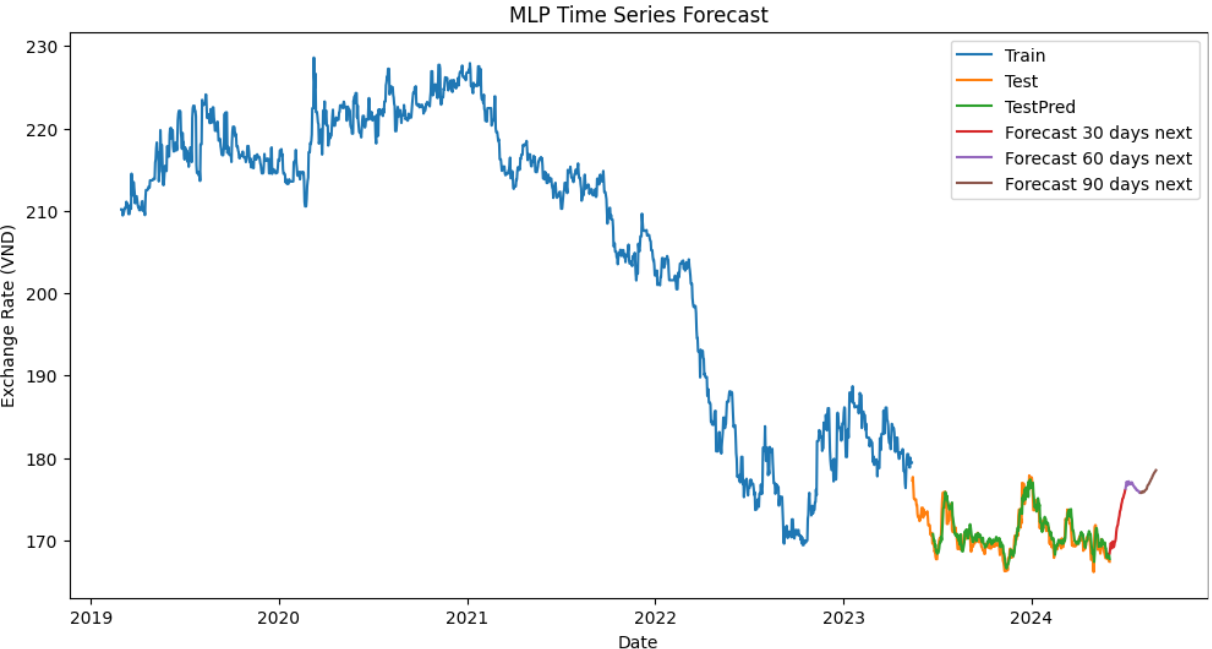
\includegraphics[width=\linewidth]{MLP/mlp_jpy_82.png}
    \caption{MLP model's result with 8:2 splitting proportion}
    \label{fig33}
  \end{minipage}
\end{figure}

\section{Conclusion}
\subsection{Summary}
In the study, we developed and evaluated several models for forecasting currency price, leveraging different statistical, deep,v and machine learning techniques. The eight models used are Linear Regression, ARIMA, Exponential Smoothing (ETS), Long Short Term Memory (LSTM), Recurrent Neural Network (RNN), Gated
Recurrent Unit (GRU), Stacking Model and Multi-layer Perceptron (MLP). The assessment and comparison of forecasting methods highlighted that each technique possessed its own advantages and drawbacks. We use metrics like RMSE, MAE and MAPE to evaluate model accuracy. By comparing these evaluation metrics, we determined that <> are well-suited for forecasting currency price. These models performed more accurately in future prices than the others. 
\subsection{Future Plans}
The above algorithms have demonstrated promising results in forecasting currency prices. However, it is necessary to enhance the model to achieve greater accuracy and reliability. To accomplish this, several key strategies can be implemented \\
\indent\textbullet\ Enhancing the accuracy of the model: It includes improving data quality by cleaning and preprocessing data before being used in the model.\\
\indent\textbullet\ Combine various Neural Network methods: It enhances the accuracy of forecasting model by combining Neural Network together. CNN-LSTM hybrid model, for instances, is effective as CNN extracts temporal features from data while LSTM captures long-term dependencies. \\
\indent\textbullet\ Research on Advanced prediction models: Find new advanced techniques such as Deep Learning and Reinforcement Learning to build more sophisticated and accurate prediction models. \\
\indent\textbullet\ Build website: Build a website that integrates various neural network models to forecast currency prices. The website can display real-time currency prices and provide features to view and forecast future prices, ensuring real-time data processing. \\

\section*{Acknowledgment}
\addcontentsline{toc}{section}{Acknowledgment}
Firstly, we send our deepest appreciation to both \textbf{Assoc. Prof. Dr. Nguyen Dinh Thuan} and \textbf{Mr. Nguyen Minh Nhut} for their invaluable guidance and insightful lessons during the research process. Their constructive feedback has enriched our research and we have not only knowledge, but also the skills needed for our careers. 
\\Secondly, this research would not have been done without the efforts and contributions of our teammates. Thank you for your continued efforts. 
\\Finally, we would like to extend our heartfelt thanks to everyone involved for their invaluable assistance, encouragement, and belief in our research. Thank you all for your invaluable assistance and encouragement.



\EOD
\printbibliography
\end{document}
